\documentclass[notheorems,compress,mathserif,table]{beamer}

\useoutertheme{tree}
\usecolortheme{whale}      % Outer color themes, 其他选择: whale, seahorse, dolphin . 换一个编译看看有什么不同.
\usecolortheme{orchid}     % Inner color themes, 其他选择: lily, orchid
\useinnertheme[shadow]{rounded} % 对 box 的设置: 圆角、有阴影.
\setbeamercolor{sidebar}{bg=blue!50} % sidebar的颜色, 50%的蓝色.
%\setbeamercolor{background canvas}{bg=blue!9} % 背景色, 9%的蓝色. 去掉下一行, 试一试这个.
\setbeamertemplate{background canvas}[vertical shading][bottom=white,top=structure.fg!25] %%背景色, 上25%的蓝, 过渡到下白.
\usefonttheme{serif}  % 字体. 个人偏好有轮廓的字体. 去掉这个设置编译, 就看到不同了.
\setbeamertemplate{navigation symbols}{}   %% 去掉页面下方默认的导航条.
%%------------------------常用宏包---------------------------------------------------------------------
%%注意, beamer 会默认使用下列宏包: amsthm, graphicx, hyperref, color, xcolor, 等等
%\usepackage{CJK}
\usepackage{ctex}
\usepackage{amsmath,amsthm,amsfonts,amssymb,bm}
\usepackage{mathrsfs}
\usepackage{subfigure} %%图形或表格并排排列
\usepackage{xmpmulti}  %%支持文中的 \multiinclude 等命令, 使 mp 文件逐帧出现. 具体讨论见 beamer 手册.
\usepackage{colortbl,dcolumn}     %% 彩色表格
%\logo{
\includegraphics[height=0.09\textwidth]{ajln.jpg}}   %左上角科大logo
%%%%%%%%%%%%%%%%%%%%%%%%%%%%%%%%%%%%%%重定义字体、字号命令 %%%%%%%%%%%%%%%%%%%%%%%%%%%%%%%%%%%%%%%%%%%%%%
%\newcommand{\songti}{\CJKfamily{song}}        % 宋体
%\newcommand{\fangsong}{\CJKfamily{fs}}        % 仿宋体
%\newcommand{\kaishu}{\CJKfamily{kai}}         % 楷体
%\newcommand{\heiti}{\CJKfamily{hei}}          % 黑体
%\newcommand{\lishu}{\CJKfamily{li}}           % 隶书
\newcommand{\youyuang}{\CJKfamily{you}}       % 幼圆
\newcommand{\sanhao}{\fontsize{16pt}{\baselineskip}\selectfont}     % 字号设置
\newcommand{\sihao}{\fontsize{14pt}{\baselineskip}\selectfont}      % 字号设置
\newcommand{\xiaosihao}{\fontsize{12pt}{\baselineskip}\selectfont}  % 字号设置
\newcommand{\wuhao}{\fontsize{10.5pt}{\baselineskip}\selectfont}    % 字号设置
\newcommand{\xiaowuhao}{\fontsize{9pt}{\baselineskip}\selectfont}   % 字号设置
\newcommand{\liuhao}{\fontsize{7.875pt}{\baselineskip}\selectfont}  % 字号设置
\newcommand{\qihao}{\fontsize{5.25pt}{\baselineskip}\selectfont}    % 字号设置
%%%%%%%%%%%%%%%%%%%%%%%%%%%%%%%%%%%%%%%%%%%%%%%%%%%%%%%%%%%%%%%%%%%%%%%%%%%%%%%%%%%%%%%%%%%%%%%%%%%%%%%%
%%----------------------- Theorems ---------------------------------------------------------------------
\newtheorem{theorem}{定理}
\newtheorem{definition}{定义}
\newtheorem{lemma}{引理}
\newtheorem{example}{例题}
\newtheorem{answer}{解:}
\newtheorem{dablock}{}
\newtheorem{jytg}{提纲}
\newtheorem{daproof}{证明}
\newtheorem{explain}{说明}
\newtheorem{summary}{小结}

\newtheorem{zhuyi}{注意}
\newtheorem{shuoming}{说明}
\newtheorem{wenti}{问题}
\newtheorem{jielun}{结论}
\newtheorem{yinli}{引理}
%%----------------------------------------------------------------------------------------------------
\title{\heiti 第1章\quad 时域离散信号与时域离散系统}
\author[\textcolor{blue}]{{\sihao\kaishu  笪邦友}}
\institute{\sihao\lishu  \textcolor{violet}{中南民族大学~~ 电子信息工程学院}}
\date{\fangsong\today} 

\begin{document}
	%  \begin{CJK*}{GBK}{kai}
\kaishu
\frame{ \titlepage }
	%%---------------------------------------------------------------------------------------------------
\section*{目录}
\frame{\kaishu\frametitle{\kaishu 目录}\tableofcontents}

%%%%%%%%%%%%%%%%%%%%%%%%%%%%%%%%%%%%%%%%%%%%%%%%%%%%%%%%%%%%%%%%%%%%%%%%%%%%%%%%%%%%%%%%%%%%%%

%%===================================================================================================
\section{1.1信号的概念}
\subsection{1.1.1信号分类}

\begin{frame}\frametitle{信号的分类}%[allowframebreaks][shrink]
\begin{dablock}
广义上讲,信号是某种随时间(或空间)变化的物理量,通常可认为是一个或几个自变量的函数。
\end{dablock}
信号可分为两大类:

\begin{enumerate}
  \item [1] \textbf{随机信号}:给定某一时间值,其函数值不确定,仅知道此信号取某一数值的概率
%  (
%              即函数为随机变量,随机信号不是一个确定的时间函数)。
%      \begin{itemize}
%        \item 本课程不考虑对随机信号的研究,但现实中的信号一般都是随机信号。
%      \end{itemize}
  \item [2]
      \textbf{确定信号}:给定某一时间值,可以确定一相应的函数值。%(信号表现为一确定的时间函数)。
       \par 确定信号中又分为:
        \begin{itemize}
          \item  \textbf{模拟信号}:在时间上和幅度上都是连续的。
          \item  \textbf{数字信号}:在时间上是离散的,在幅值上也是离散的。%(幅度离散:先取样,再量化)。
          \item  \textbf{离散信号}:在时间上是离散的,幅度上是连续的。
        \end{itemize}
        实际上,离散信号和数字信号之间的差别仅在于数字信号存在量化误差。
\end{enumerate}
\end{frame}
%%%%%%%%%%%%%%%%%%%%%%%%%%%%%%%%%%%%%%%%%%%%%%%%%%%%%%%%%%%%%%%%%%%%%%%%%%%%%%%%%%%%%%%%%%%%%%%
%
%
%
%
%
%
%%%%%%%%%%%%%%%%%%%%%%%%%%%%%%%%%%%%%%%%%%%%%%%%%%%%%%%%%%%%%%%%%%%%%%%%%%%%%%%%%%%%%%%%%%%%%%%%
\subsection{1.1.2 信号的特性}

%%%%%%%%%%%%%%%%%%%%%%%%%%%%%%%%%%%%%%%%%%%%%%%%%%%%%%%%%%%%%%%%%%%%%%%%%%%%%%%%%%%%%%%%%%%%%%
\begin{frame}\frametitle{信号的特性}%[allowframebreaks][shrink]
\begin{enumerate}
  \item \textbf{时域特性:}
      \par\qquad 也叫时间特性,包含了信号的全部信息量。其表示确定信号的时间函数,即信号随时间变化快慢的特性。
      所谓变化的快慢,则其表现为:
      \begin{enumerate}
        \item 同一形状的波形重复出现的周期短或长
        \item 信号波形本身变化速率的不同
      \end{enumerate}
  \item
      \textbf{频域特性:}
      \par\qquad 也叫频率特性,信号可以用傅里叶变换分解为许多不同频率的正弦分量,每一个
      正弦分量则以它的幅值和相位来表征,频谱同样也包含了信号的全部信息量。
\end{enumerate}
\begin{dablock}
      \textbf{两种特性之间的关系:}
      \par \quad\quad 信号的时间函数和信号频谱都是信号的表现形式,都包含了信号的全部信息,
      二者是等价的,是同一事物的不同表现形式。
\end{dablock}
\end{frame}
%%%%%%%%%%%%%%%%%%%%%%%%%%%%%%%%%%%%%%%%%%%%%%%%%%%%%%%%%%%%%%%%%%%%%%%%%%%%%%%%%%%%%%%%%%%%%%%
%%
%%
%%
%%
%%
%%
%%%%%%%%%%%%%%%%%%%%%%%%%%%%%%%%%%%%%%%%%%%%%%%%%%%%%%%%%%%%%%%%%%%%%%%%%%%%%%%%%%%%%%%%%%%%%%%
\section{1.2 时域离散信号}
\subsection{1.2.1 时域离散信号的定义}
%%%%%%%%%%%%%%%%%%%%%%%%%%%%%%%%%%%%%%%%%%%%%%%%%%%%%%%%%%%%%%%%%%%%%%%%%%%%%%%%%%%%%%%%%%%%%%
\begin{frame}[shrink]\frametitle{时域离散信号的定义}%[allowframebreaks][shrink]
\begin{definition}
对模拟信号$x_{a}(t)$进行等间隔采样,采样间隔为$T$,得到采样信号$\hat{x}_{a}(t)$
\begin{equation*}
    \hat{x}_{a}(t) = x_{a}(t)|_{t=nT} = x_{a}(nT) \quad\quad -\infty<n<\infty
\end{equation*}
这里$n$取整数。
\end{definition}

将$n$值代入$x_{a}(nT)$中,则可得到一个有序的数字序列,例如:\par
$\cdots x_{a}(-3T),x_{a}(-2T),x_{a}(-T),x_{a}(0),x_{a}(T),x_{a}(2T),x_{a}(3T),\cdots$

\end{frame}
%%%%%%%%%%%%%%%%%%%%%%%%%%%%%%%%%%%%%%%%%%%%%%%%%%%%%%%%%%%%%%%%%%%%%%%%%%%%%%%%%%%%%%%%%%%%%%%%
%%
%%
%%
%%
%%
%%
%%%%%%%%%%%%%%%%%%%%%%%%%%%%%%%%%%%%%%%%%%%%%%%%%%%%%%%%%%%%%%%%%%%%%%%%%%%%%%%%%%%%%%%%%%%%%%%%
\begin{frame}[shrink]\frametitle{时域离散信号}%[allowframebreaks][shrink]
在实际数字信号处理中,这些需要按顺序存放在存储器中,此时$nT$代表的仅是前后顺序,不代表具体采样时刻。
\begin{dablock}
\textbf{该数字序列即为时域离散信号}
\end{dablock}
为简单起见,可将公式:
$$\cdots x_{a}(-3T),x_{a}(-2T),x_{a}(-T),x_{a}(0),x_{a}(T),x_{a}(2T),x_{a}(3T),\cdots$$
简化为:
$$\cdots x(-3),x(-2),x(-1),x(0),x(1),x(2),x(3),\cdots$$
简化后的序列用集合${x(n)(-\infty<n<\infty})$表示。
\end{frame}
%%%%%%%%%%%%%%%%%%%%%%%%%%%%%%%%%%%%%%%%%%%%%%%%%%%%%%%%%%%%%%%%%%%%%%%%%%%%%%%%%%%%%%%%%%%%%%%%
%%
%%
%%
%%
%%
%%
%%%%%%%%%%%%%%%%%%%%%%%%%%%%%%%%%%%%%%%%%%%%%%%%%%%%%%%%%%%%%%%%%%%%%%%%%%%%%%%%%%%%%%%%%%%%%%%
\begin{frame}[shrink]\frametitle{区分三个不同层次的概念}%[allowframebreaks][shrink]
这里存在着三个不同层次的概念:
\begin{enumerate}
  \item [(1)]
        模拟信号$x_{a}(t)$
  \item [(2)]
        模拟信号的采样信号$x_{a}(nT)$
  \begin{itemize}
        \item
            此时为模拟信号采样点的值,且有$x_{a}(nT)= x_{a}(t)|_{t=nT}$,此时它仍是一个时间$t$的函数,只是其函数值仅在离散的时间值$t=0,\pm T,\pm 2T,\cdots$等处被定义。
      \end{itemize}
        \item [(3)]从更抽象的层次看,时域离散信号可看作一个序列,这时有$x(n)=x_{a}(nT)$,从更一般的情况来看,$n$可以只代表顺序,而不仅仅局限于时间变量。
\end{enumerate}
\end{frame}
%%%%%%%%%%%%%%%%%%%%%%%%%%%%%%%%%%%%%%%%%%%%%%%%%%%%%%%%%%%%%%%%%%%%%%%%%%%%%%%%%%%%%%%%%%%%%%%%
%%
%%
%%
%%
%%
%%
%%%%%%%%%%%%%%%%%%%%%%%%%%%%%%%%%%%%%%%%%%%%%%%%%%%%%%%%%%%%%%%%%%%%%%%%%%%%%%%%%%%%%%%%%%%%%%%%
\begin{frame}[shrink]\frametitle{几点说明}%[allowframebreaks][shrink]
需要说明几点:

\begin{itemize}
  \item $n$取整数值,对于非整数$n$,序列$x(n)$无意义。\par (但并不为0)
  \item 在数值上,有:$$x(n)=x_{a}(nT)=x_{a}(t)|_{t=nT}$$
        这一点非常重要,以后多次用到。
  \item 离散序列是从负无穷到正无穷的。即:$-\infty<n<\infty$
\end{itemize}
\end{frame}
%%%%%%%%%%%%%%%%%%%%%%%%%%%%%%%%%%%%%%%%%%%%%%%%%%%%%%%%%%%%%%%%%%%%%%%%%%%%%%%%%%%%%%%%%%%%%%%
%
%
%
%
%
%
%%%%%%%%%%%%%%%%%%%%%%%%%%%%%%%%%%%%%%%%%%%%%%%%%%%%%%%%%%%%%%%%%%%%%%%%%%%%%%%%%%%%%%%%%%%%%%%
\begin{frame}[shrink]\frametitle{时域离散信号的表示方法}%[allowframebreaks][shrink]
\begin{enumerate}
  \item 公式法: 如$x(n)=sin(\omega n)$表示一正弦离散信号。
  \item 图示法:用图形表示序列,是一种很直观的方法。
%        如 $x(n)=sin(\omega n)$ 可用以下图形表示。
        \begin{figure}[h]
          \centering
          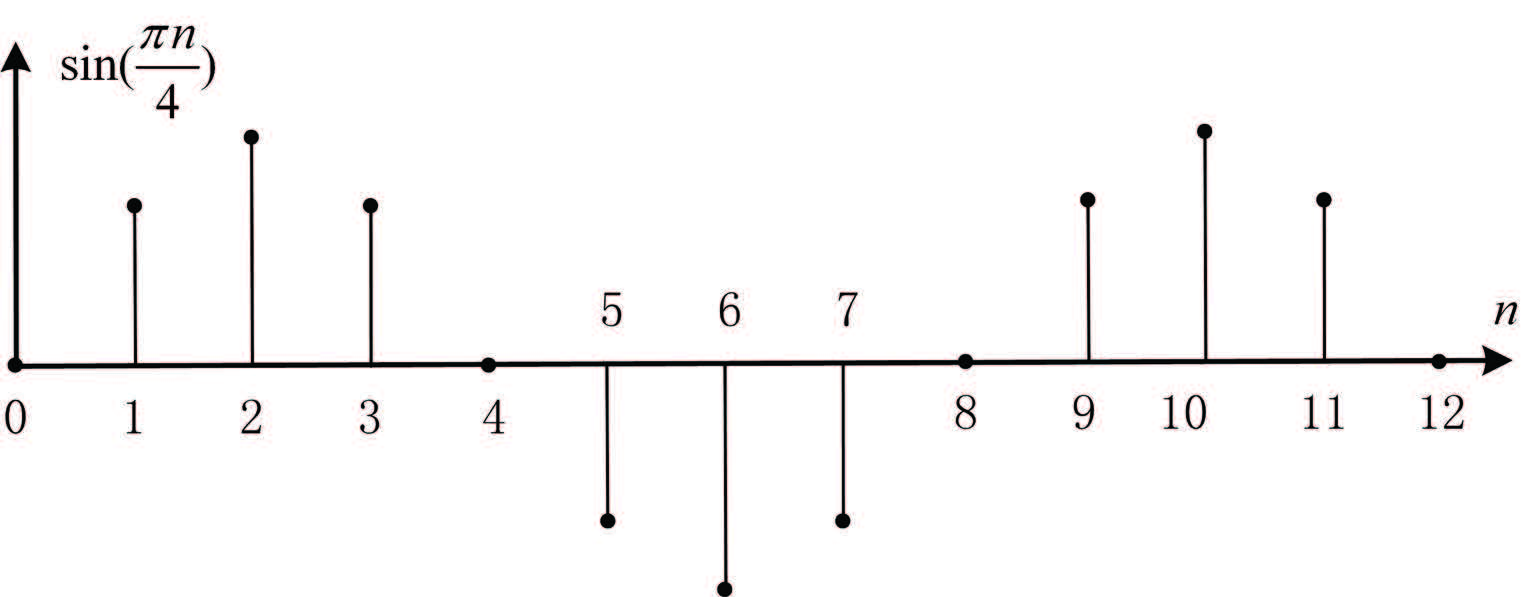
\includegraphics[width=0.6\textwidth]{zhengxianxulie.jpg}\\
          %\caption{正弦序列}
          %\label{}
        \end{figure}
  \item 集合法:
        因为时域离散信号是一个有序的数的集合。用集合符号表示,可用集合符号表示。
        如$$x(n) = \{\cdots,0,\underline{1},2,3,4,3,2,1,0,\cdots\}$$
        集合中有下划线的元素表示n=0时刻的采样点。
\end{enumerate}
\end{frame}
%%%%%%%%%%%%%%%%%%%%%%%%%%%%%%%%%%%%%%%%%%%%%%%%%%%%%%%%%%%%%%%%%%%%%%%%%%%%%%%%%%%%%%%%%%%%%%






%%%%%%%%%%%%%%%%%%%%%%%%%%%%%%%%%%%%%%%%%%%%%%%%%%%%%%%%%%%%%%%%%%%%%%%%%%%%%%%%%%%%%%%%%%%%%%%
\subsection{1.2.2 序列的运算}

\begin{frame}[shrink]\frametitle{序列的运算}%[allowframebreaks][shrink]
\begin{dablock}
\begin{enumerate}
  \item [(1)]  \textbf{乘法:} 同序号的序列值逐项对应相乘, 表示为:\par \qquad\qquad $y(n) = x(n) \cdot h(n)$
  \item [(2)] \textbf{加法:} 同序号的序列值逐项对应相加, 表示为:\par \qquad\qquad $y(n) = x(n) + h(n)$
  \item [(3)] \textbf{卷积和:} 设两序列为$x(n)$和$h(n)$,则$x(n)$和$h(n)$的卷积和\par
  \qquad \qquad 定义为:
        \begin{equation*}
            y(n) = x(n)*h(n) = \sum_{m=-\infty}^{\infty}x(m)h(n-m)
        \end{equation*}
\end{enumerate}
\end{dablock}
\begin{itemize}
  \item 卷积和是求离散线性时不变系统输出响应(零状态响应)的主要方法。
  \item 卷积和的运算可分为四步:翻转、移位、相乘、相加。
\end{itemize}



\end{frame}
%%%%%%%%%%%%%%%%%%%%%%%%%%%%%%%%%%%%%%%%%%%%%%%%%%%%%%%%%%%%%%%%%%%%%%%%%%%%%%%%%%%%%%%%%%%%%%%
%
%
%
%
%
%
%%%%%%%%%%%%%%%%%%%%%%%%%%%%%%%%%%%%%%%%%%%%%%%%%%%%%%%%%%%%%%%%%%%%%%%%%%%%%%%%%%%%%%%%%%%%%%%
\begin{frame}[shrink]\frametitle{序列的变换}
  \begin{enumerate}
    \item \textbf{移位(延迟)}:\par 对序列$x(n)$,当$m$为正整数时,\par 则$x(n-m)$是指序列$x(n)$逐项依次延
        时(右移)$m$位。而$x(n+m)$是指序列$x(n)$逐项依次超前(左移)$m$ 位。
    \item \textbf{翻转:}  \par 如果序列为$x(n)$,则$x(-n)$是以$n=0$的纵轴为对称轴将序列$x(n)$加以翻转。
    \item \textbf{尺度变换:} \par 对序列$x(n)$,其时间尺度变换序列为$x(mn)$或$x(\frac{n}{m})$,其中m 为正整数。
        前者称为抽取,后者称为插值
        \begin{itemize}
          \item \textbf{注意}:离散信号的尺度变化与模拟信号的尺度变换有较大不同,离散信号的尺度
        实际为抽取或插值,跟原序列相比,是两个不同的序列。
        \end{itemize}

\end{enumerate}
\end{frame}

%\subsubsection*{尺度变换}尺度变换举例
%\begin{frame}[shrink]\frametitle{}%[allowframebreaks][shrink]
%\textbf{例如},对于如下离散信号序列,\par $x(n)= {\cdots,0,-2,0.5,\underline{2},1,1.5,0,-1,2,1,0,\cdots}$, 抽取前$x(n)$图形表示如下:
%\begin{figure}[h]
%  \centering
%  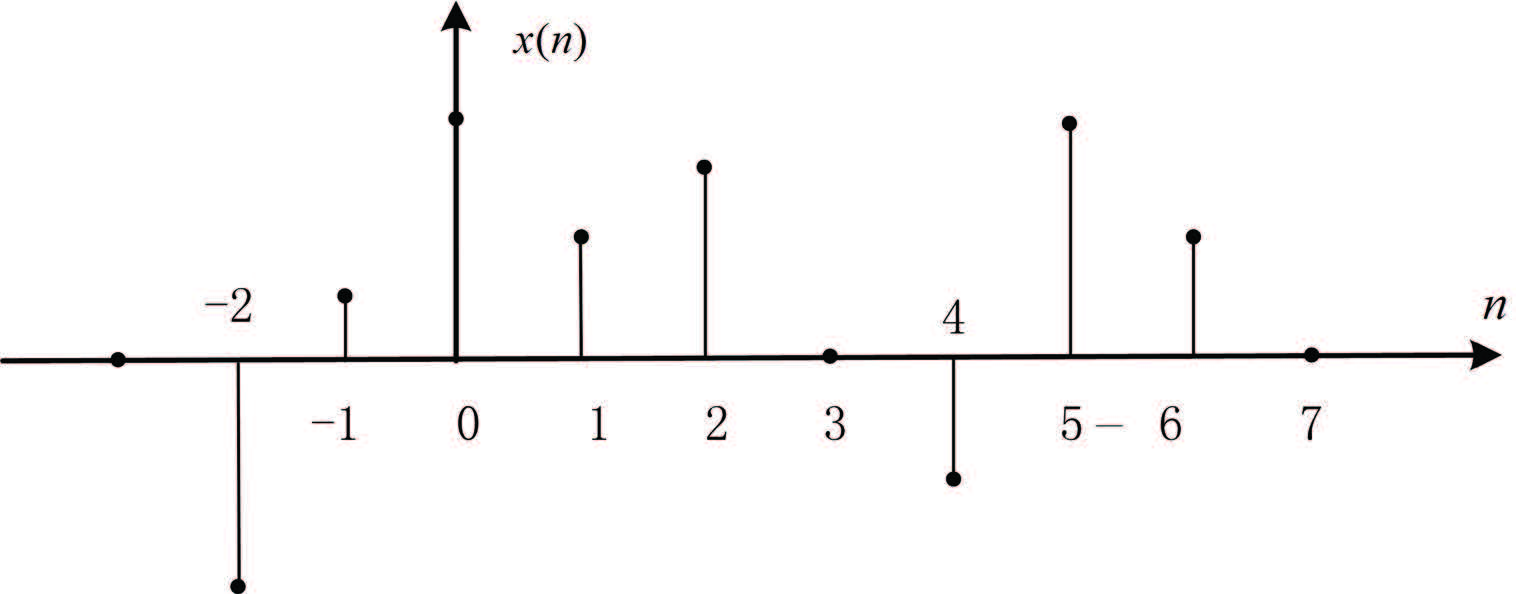
\includegraphics[width=0.5\textwidth]{yiweijiaquanhe.jpg}\\
%  %\caption{用单位采样序列移位加权和表示序列}
%  %\label{}
%\end{figure}
%
%$x(2n) = {\cdots,0,-2,\underline{2},1.5,-1,1,0,\cdots,}$,抽取后$x(2n)$图形表示如下:
%\begin{figure}[h]
%  \centering
%  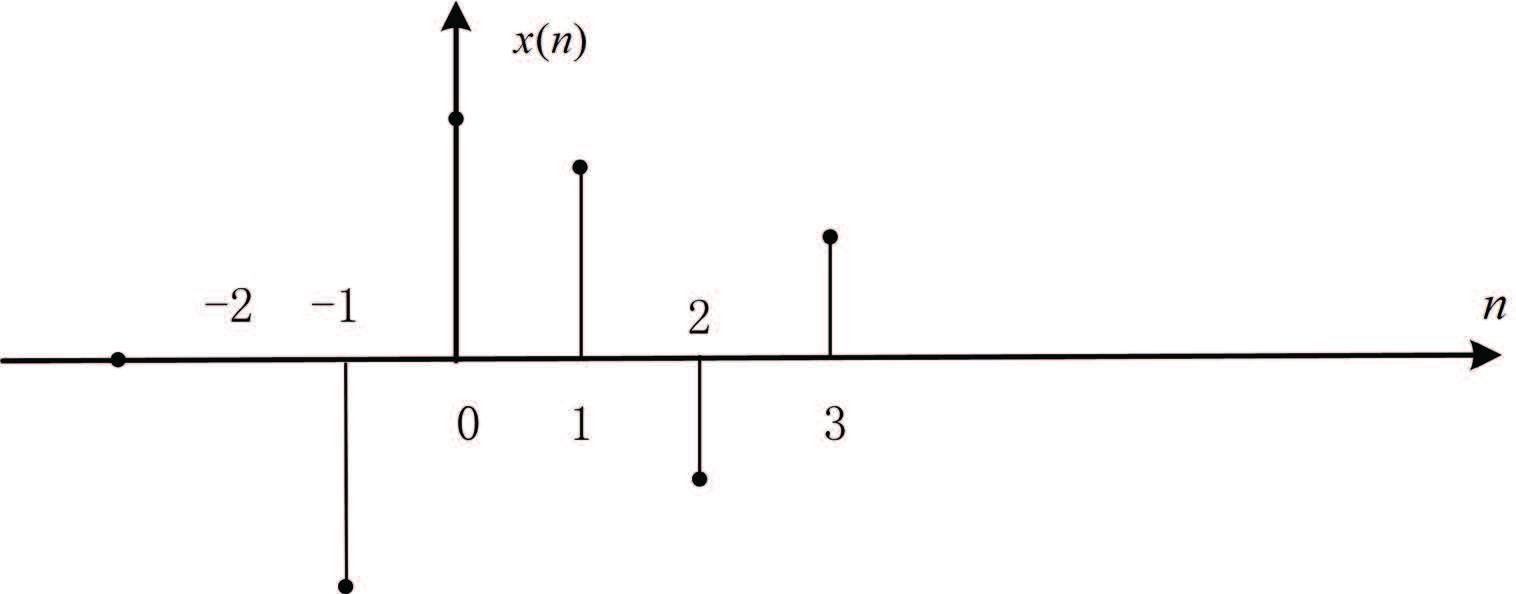
\includegraphics[width=0.5\textwidth]{chouquhou.jpg}\\
%  %\caption{用单位采样序列移位加权和表示序列}
%  %\label{}
%\end{figure}
%
%\end{frame}
%%%%%%%%%%%%%%%%%%%%%%%%%%%%%%%%%%%%%%%%%%%%%%%%%%%%%%%%%%%%%%%%%%%%%%%%%%%%%%%%%%%%%%%%%%%%%%%
%
%
%
%
%
%
%%%%%%%%%%%%%%%%%%%%%%%%%%%%%%%%%%%%%%%%%%%%%%%%%%%%%%%%%%%%%%%%%%%%%%%%%%%%%%%%%%%%%%%%%%%%%%%
\subsection{1.2.3 常见的典型序列}
%%%%%%%%%%%%%%%%%%%%%%%%%%%%%%%%%%%%%%%%%%%%%%%%%%%%%%%%%%%%%%%%%%%%%%%%%%%%%%%%%%%%%%%%%%%%%%
\begin{frame}\frametitle{常见的典型序列}%[allowframebreaks][shrink]
\begin{enumerate}
  \item[(1)] 单位采样序列$\delta(n)$
  \item[(2)] 单位阶跃序列$u(n)$
  \item[(3)] 矩形序列$R_{N}(n)$
  \item[(4)] 实指数序列
  \item[(5)] 正弦序列
  \item[(6)] 复指数序列
\end{enumerate}
\end{frame}
%%%%%%%%%%%%%%%%%%%%%%%%%%%%%%%%%%%%%%%%%%%%%%%%%%%%%%%%%%%%%%%%%%%%%%%%%%%%%%%%%%%%%%%%%%%%%%%
%
%
%
%
%
%
%%%%%%%%%%%%%%%%%%%%%%%%%%%%%%%%%%%%%%%%%%%%%%%%%%%%%%%%%%%%%%%%%%%%%%%%%%%%%%%%%%%%%%%%%%%%%%%
\subsubsection*{单位采样序列$\delta(n)$}
%%%%%%%%%%%%%%%%%%%%%%%%%%%%%%%%%%%%%%%%%%%%%%%%%%%%%%%%%%%%%%%%%%%%%%%%%%%%%%%%%%%%%%%%%%%%%%
\begin{frame}[shrink]\frametitle{单位脉冲序列$\delta(n)$}%[allowframebreaks][shrink]
\begin{definition}
\begin{equation*}\label{fol:delta}
     \delta(n)= \left\{\begin{array}
     {r@{,\quad}l}
     1&\mbox{$n=0$}\\0&\mbox{$n\neq 0$}
    \end{array} \right.
\end{equation*}
\end{definition}
也称为单位脉冲序列,与模拟信号中的单位冲击函数$\delta(t)$相对应,
不同处在于,$\delta(n)$是一个普通函数,而$\delta(t)$是一个奇异函数。
\begin{figure}[h]
  % Requires \usepackage{graphicx}
  \centering
  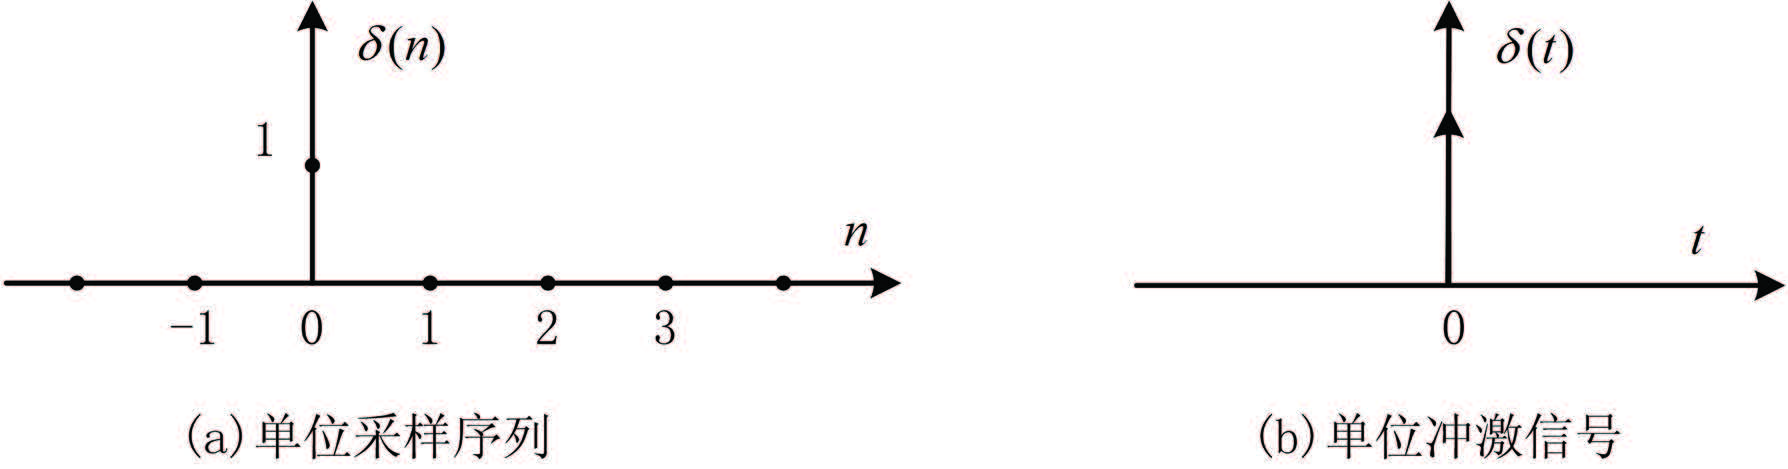
\includegraphics[width=0.8\textwidth]{danweicaiyang.jpg}
  %\caption{单位采样序列和单位冲激信号}
  %\label{}
\end{figure}
\begin{itemize}
  \item [\textbf{注意:}]单位采样序列的长度是从$-\infty$到$\infty$,仅$x(0)=1$,其余处值为0。
\end{itemize}
\end{frame}
%%%%%%%%%%%%%%%%%%%%%%%%%%%%%%%%%%%%%%%%%%%%%%%%%%%%%%%%%%%%%%%%%%%%%%%%%%%%%%%%%%%%%%%%%%%%%%%
%
%
%
%
%
%
%%%%%%%%%%%%%%%%%%%%%%%%%%%%%%%%%%%%%%%%%%%%%%%%%%%%%%%%%%%%%%%%%%%%%%%%%%%%%%%%%%%%%%%%%%%%%%%
\subsubsection*{单位阶跃序列$u(n)$}
%%%%%%%%%%%%%%%%%%%%%%%%%%%%%%%%%%%%%%%%%%%%%%%%%%%%%%%%%%%%%%%%%%%%%%%%%%%%%%%%%%%%%%%%%%%%%%
\begin{frame}[shrink]\frametitle{单位阶跃序列$u(n)$}%[allowframebreaks][shrink]
\begin{definition}
\begin{equation*}
     u(n)= \left\{\begin{array}
     {r@{,\quad}l}
     1&\mbox{$n\geq0$}\\0&\mbox{$n<0$}
    \end{array} \right.
\end{equation*}
\end{definition}
单位阶跃信号类似于模拟信号中的单位阶跃函数$u(t)$,其图形如下:
\begin{figure}[h]
  % Requires \usepackage{graphicx}
  \centering
  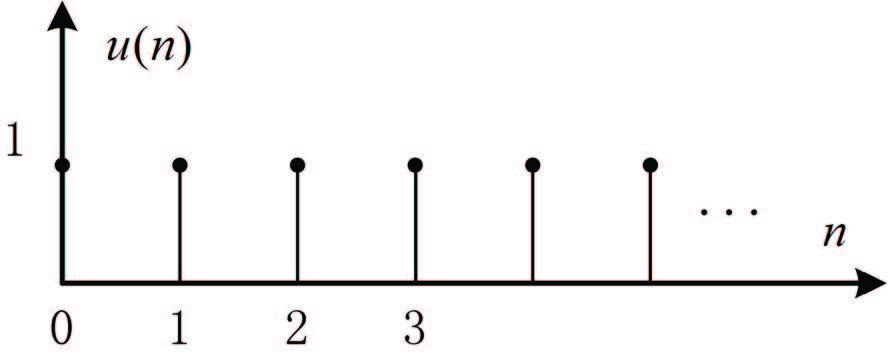
\includegraphics[width=0.50\textwidth]{danweijieyue.jpg}
  %\caption{单位阶跃序列}
  %\label{}
\end{figure}
%\vspace{-0.5cm}

\end{frame}
%%%%%%%%%%%%%%%%%%%%%%%%%%%%%%%%%%%%%%%%%%%%%%%%%%%%%%%%%%%%%%%%%%%%%%%%%%%%%%%%%%%%%%%%%%%%%%%
%
%
%
%
%
%
%%%%%%%%%%%%%%%%%%%%%%%%%%%%%%%%%%%%%%%%%%%%%%%%%%%%%%%%%%%%%%%%%%%%%%%%%%%%%%%%%%%%%%%%%%%%%%%
\begin{frame}\frametitle{单位阶跃序列}%[allowframebreaks][shrink]
因为
\begin{equation*}\label{fol:delta}
     u(n)= \left\{\begin{array}
     {r@{,\quad}l}
     1&\mbox{$n\geq0$}\\0&\mbox{$n<0$}
    \end{array} \right.
\end{equation*}
显然有:%\vspace{-0.5cm}
%\emph{\textbf{(利用图形表示法推导3个公式)}}
\begin{equation*}%\label{}
    \delta(n)= u(n)-u(n-1)
\end{equation*}
\vspace{-0.5cm}
\begin{equation*}%\label{}
    u(n)= \sum_{k=0}^{\infty}\delta(n-k)
\end{equation*}
$\quad\quad\quad\quad$令$m=n-k$,代入上式得到:
\begin{equation*}%\label{}
    u(n)= \sum_{m=-\infty}^{n}\delta(m)
\end{equation*}
\end{frame}
%%%%%%%%%%%%%%%%%%%%%%%%%%%%%%%%%%%%%%%%%%%%%%%%%%%%%%%%%%%%%%%%%%%%%%%%%%%%%%%%%%%%%%%%%%%%%%%
%
%
%
%
%
%
%%%%%%%%%%%%%%%%%%%%%%%%%%%%%%%%%%%%%%%%%%%%%%%%%%%%%%%%%%%%%%%%%%%%%%%%%%%%%%%%%%%%%%%%%%%%%%%
\subsubsection*{矩形序列$R_{N}(n)$}
%%%%%%%%%%%%%%%%%%%%%%%%%%%%%%%%%%%%%%%%%%%%%%%%%%%%%%%%%%%%%%%%%%%%%%%%%%%%%%%%%%%%%%%%%%%%%%
\begin{frame}\frametitle{矩形序列$R_{N}(n)$}%[allowframebreaks][shrink]
\begin{definition}
\begin{equation*}
     R_{N}(n)= \left\{\begin{array}
     {r@{,\quad}l}
     1&\mbox{$0\leq n\leq N-1$}\\0&\mbox{其他}
    \end{array} \right.
\end{equation*}
上式中$N$称为矩形序列的长度。
\end{definition}
例如,当$N=4 $时,$R_{N}(n)$的波形如下图所示。
\begin{figure}[h]
  \centering
  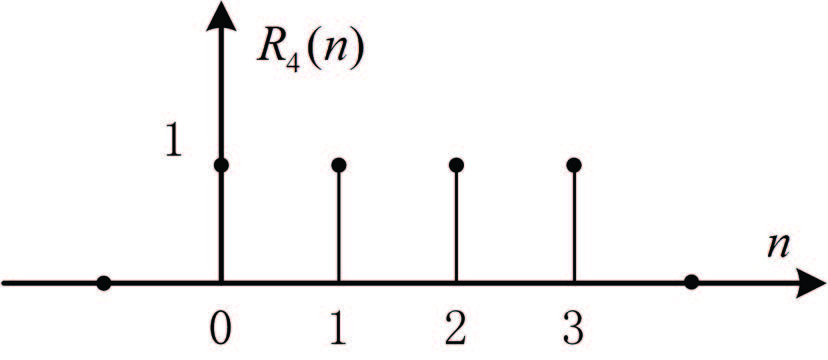
\includegraphics[width=0.5\textwidth]{juxing.jpg}
  %\caption{矩形序列}
\end{figure}
%\vspace{-0.5cm}
\begin{center}
显然有$\quad\quad R_{N}(n) = u(n)- u(n-N) $
\end{center}
\end{frame}
%%%%%%%%%%%%%%%%%%%%%%%%%%%%%%%%%%%%%%%%%%%%%%%%%%%%%%%%%%%%%%%%%%%%%%%%%%%%%%%%%%%%%%%%%%%%%%%%

\subsubsection*{实指数序列}
%%%%%%%%%%%%%%%%%%%%%%%%%%%%%%%%%%%%%%%%%%%%%%%%%%%%%%%%%%%%%%%%%%%%%%%%%%%%%%%%%%%%%%%%%%%%%%
\begin{frame}\frametitle{实指数序列}%[allowframebreaks][shrink]
\begin{definition}
\begin{equation*}
    x(n) = a^{n}u(n), \quad\quad a \in R
\end{equation*}
如果$|a|<1$,$x(n)$为收敛序列,如$|a|>1$,$x(n)$为发散序列。
\end{definition}
其波形如下所示。
\begin{figure}[h]
  % Requires \usepackage{graphicx}
  \centering
  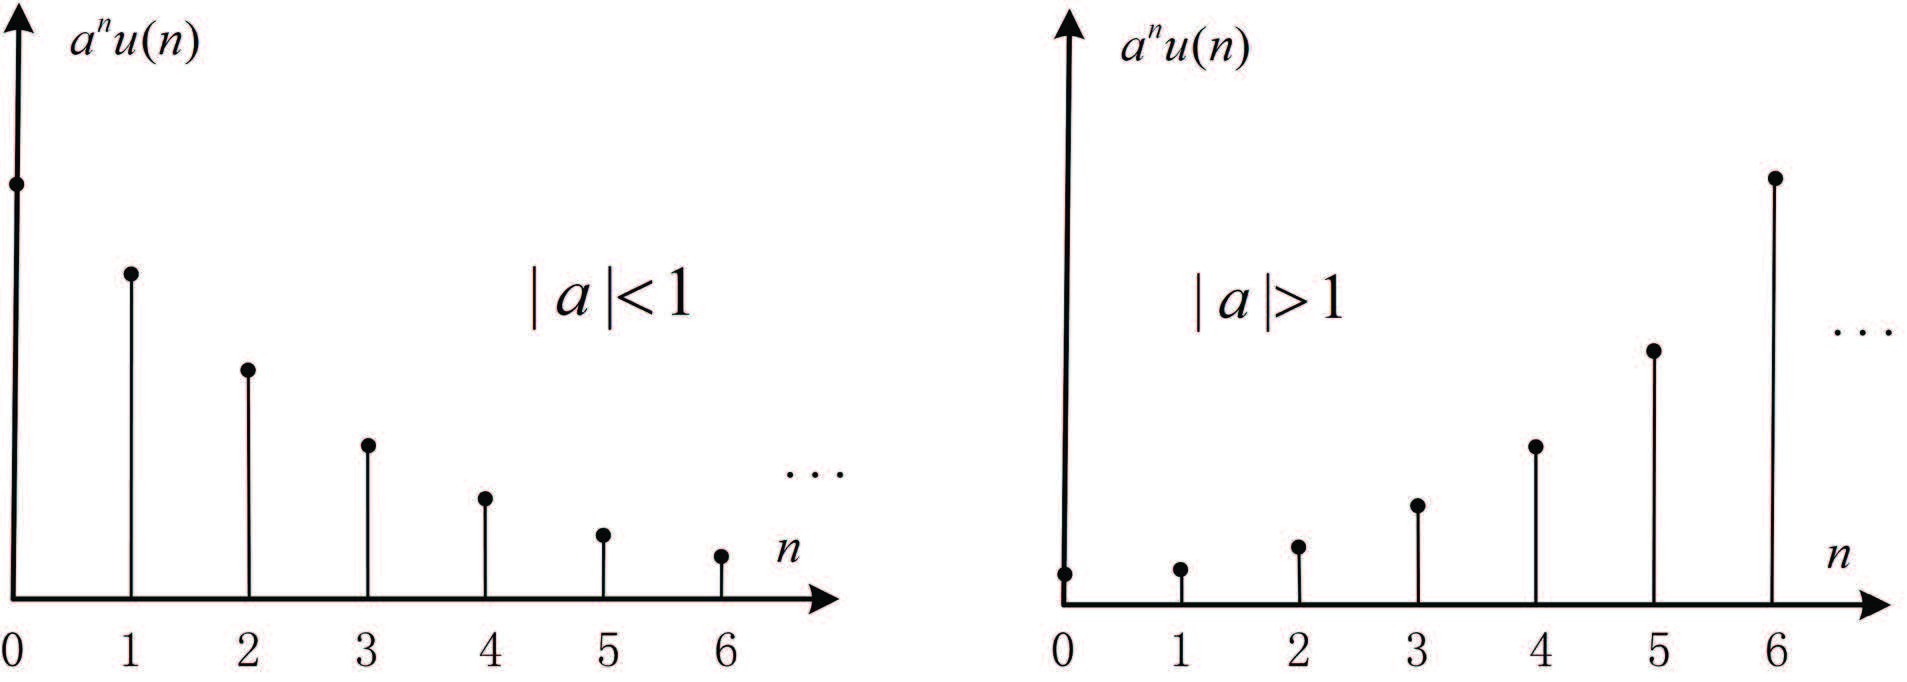
\includegraphics[width=0.75\textwidth]{shizhishu.jpg}\\
  %\caption{实指数序列}
  %\label{}
\end{figure}
%\vspace{-0.5cm}
\begin{itemize}
  \item\textbf{ 注意}:当$n<0$ 时,$x(n)=0$。
\end{itemize}
\end{frame}
%%%%%%%%%%%%%%%%%%%%%%%%%%%%%%%%%%%%%%%%%%%%%%%%%%%%%%%%%%%%%%%%%%%%%%%%%%%%%%%%%%%%%%%%%%%%%%%

\subsubsection*{正弦序列}
%%%%%%%%%%%%%%%%%%%%%%%%%%%%%%%%%%%%%%%%%%%%%%%%%%%%%%%%%%%%%%%%%%%%%%%%%%%%%%%%%%%%%%%%%%%%%%
\begin{frame}\frametitle{正弦序列}%[allowframebreaks][shrink]
\begin{definition}
\begin{equation*}
    x(n) = sin(\omega n)
\end{equation*}

式中$\omega$为正弦序列的数字域频率,单位为弧度。
\emph{表示序列变化的速率,或两个相邻序列值之间变化的弧度数。}
\end{definition}
$$\mbox{如}\qquad\qquad x(n) = sin(\frac{\pi}{4}n)\qquad \omega = \frac{\pi}{4}\qquad\qquad\qquad$$

\begin{figure}[h]
  \centering
  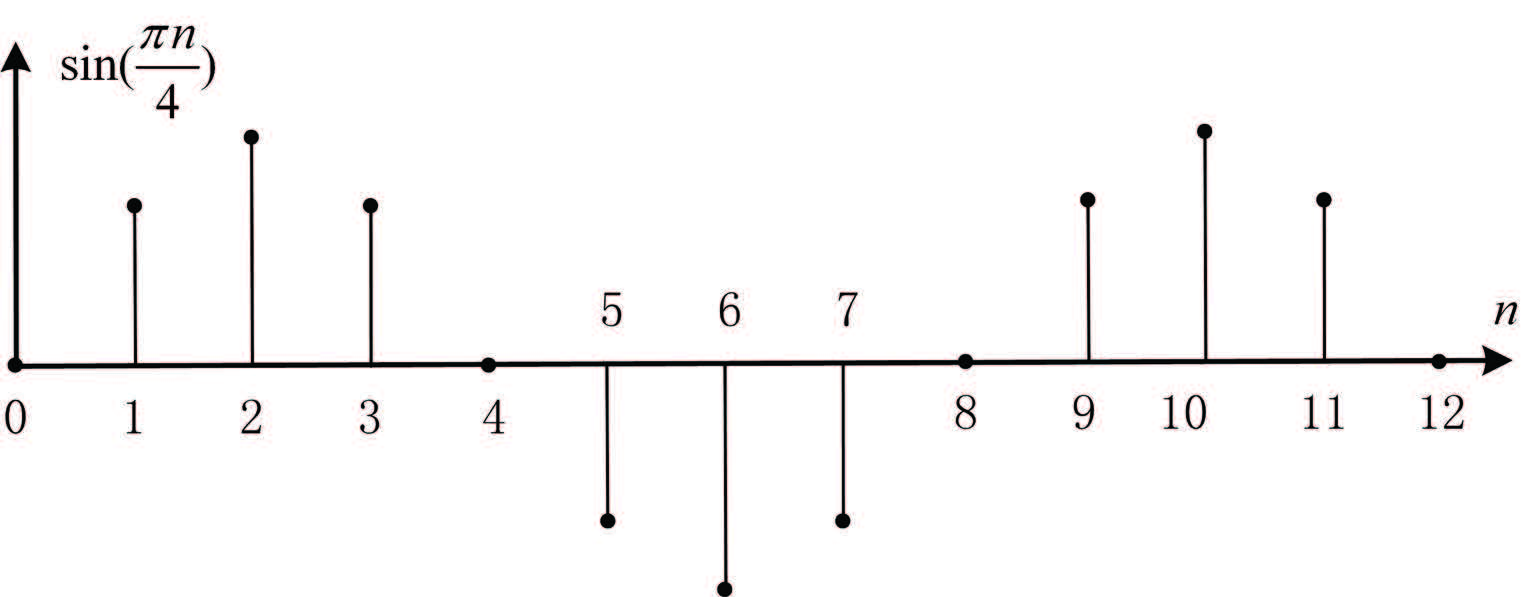
\includegraphics[width=0.6\textwidth]{zhengxianxulie.jpg}\\
  %\caption{正弦序列}
  %\label{}
\end{figure}
\end{frame}
%%%%%%%%%%%%%%%%%%%%%%%%%%%%%%%%%%%%%%%%%%%%%%%%%%%%%%%%%%%%%%%%%%%%%%%%%%%%%%%%%%%%%%%%%%%%%%%


%%%%%%%%%%%%%%%%%%%%%%%%%%%%%%%%%%%%%%%%%%%%%%%%%%%%%%%%%%%%%%%%%%%%%%%%%%%%%%%%%%%%%%%%%%%%%%
\begin{frame}[shrink]\frametitle{数字频率$\omega$和模拟信号中的角频率$\Omega$的关系}%[allowframebreaks][shrink]
%\begin{quote}
%\textbf{那么数字频率和模拟信号中的角频率有什么关系呢?}
%\end{quote}

假设$x(n)=sin(\omega n)$是由模拟信号$x_{a}(t)= sin(\Omega t)$采样得到的,这里
$\Omega$为模拟角频率,单位是:弧度/秒。
$$\mbox{因为:}\qquad x(n) = x_{a}(nT) = x_{a}(t)|_{t=nT}\qquad\qquad\qquad$$
$$\mbox{所以:}\qquad x(n) =  sin(\Omega t)|_{t=nT} = sin(\Omega nT)\qquad\qquad$$
\quad\quad 与$x(n) = sin(\omega n)$进行对比,可得:
$$
    \omega = \Omega T = \frac{\Omega}{f_{s}}$$
\begin{itemize}
  \item 这里$T$是采样间隔,$f_{s} =\frac{1}{T}$是采样频率
\end{itemize}

即:数字域频率是模拟角频率对采样频率$f_{s}$的归一化频率。
\end{frame}
%%%%%%%%%%%%%%%%%%%%%%%%%%%%%%%%%%%%%%%%%%%%%%%%%%%%%%%%%%%%%%%%%%%%%%%%%%%%%%%%%%%%%%%%%%%%%%%


%%%%%%%%%%%%%%%%%%%%%%%%%%%%%%%%%%%%%%%%%%%%%%%%%%%%%%%%%%%%%%%%%%%%%%%%%%%%%%%%%%%%%%%%%%%%%%
\begin{frame}[shrink]\frametitle{结论}%[allowframebreaks][shrink]
设$x(n)=sin(\omega n)$是由模拟信号$x_{a}(t)= sin(\Omega t)$采样得到,则:
$$    \omega = \Omega T = \frac{\Omega}{f_{s}}$$
\begin{itemize}
  \item 这里$T$是采样间隔,$f_{s} =\frac{1}{T}$是采样频率
\end{itemize}
\begin{dablock}
即:数字域频率是模拟角频率对采样频率$f_{s}$的归一化频率。
\end{dablock}
今后
\begin{enumerate}
  \item [(1)] $\omega$表示数字频率
  \item [(2)] $\Omega$或$f$表示模拟角频率或模拟频率。
\end{enumerate}

正弦序列在数字信号处理学科中具有重要的地位,同学们需要熟练掌握正弦序列的相关知识。
\end{frame}
%%%%%%%%%%%%%%%%%%%%%%%%%%%%%%%%%%%%%%%%%%%%%%%%%%%%%%%%%%%%%%%%%%%%%%%%%%%%%%%%%%%%%%%%%%%%%%%

\subsubsection*{复指数序列}
%%%%%%%%%%%%%%%%%%%%%%%%%%%%%%%%%%%%%%%%%%%%%%%%%%%%%%%%%%%%%%%%%%%%%%%%%%%%%%%%%%%%%%%%%%%%%%
\begin{frame}[shrink]\frametitle{复指数序列}%[allowframebreaks][shrink]
\begin{definition}
复指数序列用下式表示:
$$ x(n) = e^{(\sigma + j\omega_{0})n}$$
式中,$\omega_0$ 为数字域频率。
\end{definition}
%复指数序列又可写成:$$x(n) = e^{\sigma n}e^{j\omega_{0}n} = e^{\sigma n}cos(\omega_{0}n)+je^{\sigma n}sin(\omega_{0}n)$$

特别,当$\sigma =0$时,有$$x(n)=e^{j\omega_{0}n}$$

由于$n$取整数,显然:
$$x(n) = e^{(\sigma+j\omega_{0})n} = e^{(\sigma +j(\omega_{0}+2\pi M))n}$$

即:复指数序列的频率$\omega$以$2\pi$为周期,研究该序列频率特性时,只需考虑$2\pi$范围
内即可。
%\subsubsection{小结}

\end{frame}
%%%%%%%%%%%%%%%%%%%%%%%%%%%%%%%%%%%%%%%%%%%%%%%%%%%%%%%%%%%%%%%%%%%%%%%%%%%%%%%%%%%%%%%%%%%%%%%
\subsection{两个重要问题}
\subsubsection*{序列的周期性}
%%%%%%%%%%%%%%%%%%%%%%%%%%%%%%%%%%%%%%%%%%%%%%%%%%%%%%%%%%%%%%%%%%%%%%%%%%%%%%%%%%%%%%%%%%%%%
\begin{frame}[shrink]\frametitle{序列的周期性}%[allowframebreaks][shrink]


周期性是信号的一个重要特性,有必要单独考察离散信号序列的周期性。
\begin{definition}
如
\begin{equation*}
    x(n) = x(n+N)\quad\quad  -\infty <n<\infty
\end{equation*}


且$N$是满足该式的最小正整数,则称$x(n)$是以N为周期的周期序列。
\end{definition}

例如:$$x(n) = sin(n\pi/4) = sin\Big(\frac{\pi}{4}(n+8)\Big)$$

   是以8为周期的周期序列。
\end{frame}
%%%%%%%%%%%%%%%%%%%%%%%%%%%%%%%%%%%%%%%%%%%%%%%%%%%%%%%%%%%%%%%%%%%%%%%%%%%%%%%%%%%%%%%%%%%%%%%


%%%%%%%%%%%%%%%%%%%%%%%%%%%%%%%%%%%%%%%%%%%%%%%%%%%%%%%%%%%%%%%%%%%%%%%%%%%%%%%%%%%%%%%%%%%%%%%

\subsubsection*{正弦序列的周期性}
%%%%%%%%%%%%%%%%%%%%%%%%%%%%%%%%%%%%%%%%%%%%%%%%%%%%%%%%%%%%%%%%%%%%%%%%%%%%%%%%%%%%%%%%%%%%%%%

\begin{frame}\frametitle{正弦序列的周期性}%[allowframebreaks][shrink]
在各种周期序列中,正弦序列具有最重要的地位。

因此,我们下面详细讨论一下正弦序列的周期性。


\begin{enumerate}
  \item 对于模拟信号$sin(x)$来说,其总是一个周期信号
  \item 但对其采样后,得到的离散正弦序列并不总是满足周期性。
\end{enumerate}
\quad\newline\newline\quad\
问题:
\emph{什么情况下正弦序列是周期函数呢?}
\end{frame}
%%%%%%%%%%%%%%%%%%%%%%%%%%%%%%%%%%%%%%%%%%%%%%%%%%%%%%%%%%%%%%%%%%%%%%%%%%%%%%%%%%%%%%%%%%%%%%%

%%%%%%%%%%%%%%%%%%%%%%%%%%%%%%%%%%%%%%%%%%%%%%%%%%%%%%%%%%%%%%%%%%%%%%%%%%%%%%%%%%%%%%%%%%%%%%%

\begin{frame}\frametitle{正弦序列的周期性}%[allowframebreaks][shrink]
一般正弦序列如下:
$$x(n) = sin(\omega n) = sin(\omega(n+\frac{2\pi}{\omega}))$$
\begin{jielun}
\begin{enumerate}
  \item [(1)]
      若$\frac{2\pi}{\omega}$为整数,则$ T= \frac{2\pi}{\omega}$。
      \par 例如序列$x(n)=sin(\frac{\pi}{4}  n)$,其周期为$\frac{2\pi}{\pi/4}=8$
  \item [(2)]
      若$\frac{2\pi}{\omega}$为有理数,且$\frac{2\pi}{\omega}= \frac{P}{Q}$,
      这里$P$与$Q$互为素数的整数,则周期为$T=P$。
      例如:$x(n)=sin(6\pi n/7)$,$2\pi/(6\pi/7)=7/3$,其周期为7。
  \item [(3)]
      若$\frac{2\pi}{\omega}$为无理数,则其为非周期序列。
\end{enumerate}
\end{jielun}
\end{frame}
%%%%%%%%%%%%%%%%%%%%%%%%%%%%%%%%%%%%%%%%%%%%%%%%%%%%%%%%%%%%%%%%%%%%%%%%%%%%%%%%%%%%%%%%%%%%%%%



%%%%%%%%%%%%%%%%%%%%%%%%%%%%%%%%%%%%%%%%%%%%%%%%%%%%%%%%%%%%%%%%%%%%%%%%%%%%%%%%%%%%%%%%%%%%%%
\begin{frame}\frametitle{正弦序列周期举例}%[allowframebreaks][shrink]
\begin{example}

$x(n) = sin(\frac{\pi}{8}n)\:\:\quad\quad \frac{2\pi}{\omega} =\frac{2\pi}{\pi/8}=16           \:\quad\quad T = 16  $
\par\quad\newline\quad
$x(n) = sin(8\pi n)        \quad\:\quad \frac{2\pi}{\omega} =\frac{2\pi}{8\pi}= \frac{1}{8}    \qquad\quad T = 1  $
\par\quad\newline\quad
$x(n) = sin(\frac{5\pi}{2}n) \quad\:\:\quad \frac{2\pi}{\omega} =\frac{2\pi}{5\pi/2}=\frac{4}{5} \quad\quad T = 4  $
\par\quad\newline\quad
$x(n) = sin(5n)            \quad\quad\quad \frac{2\pi}{\omega} =\frac{2\pi}{5}=\frac{2}{5}\pi      \quad\quad\mbox{非周期序列}$
\end{example}
\end{frame}
%%%%%%%%%%%%%%%%%%%%%%%%%%%%%%%%%%%%%%%%%%%%%%%%%%%%%%%%%%%%%%%%%%%%%%%%%%%%%%%%%%%%%%%%%%%%%%%


\subsubsection*{用单位采样序列来表示任意序列}
%%%%%%%%%%%%%%%%%%%%%%%%%%%%%%%%%%%%%%%%%%%%%%%%%%%%%%%%%%%%%%%%%%%%%%%%%%%%%%%%%%%%%%%%%%%%%%
\begin{frame}\frametitle{用单位采样序列来表示任意序列}%[allowframebreaks][shrink]


任意序列利用单位采样序列的移位加权和表示,即
\begin{equation*}
    x(n) = \sum_{m=-\infty}^{\infty}x(m)\delta(n-m)
\end{equation*}
这种任意序列的表示方法,在信号分析中是个非常有用的公式。
\end{frame}
%%%%%%%%%%%%%%%%%%%%%%%%%%%%%%%%%%%%%%%%%%%%%%%%%%%%%%%%%%%%%%%%%%%%%%%%%%%%%%%%%%%%%%%%%%%%%%%


%%%%%%%%%%%%%%%%%%%%%%%%%%%%%%%%%%%%%%%%%%%%%%%%%%%%%%%%%%%%%%%%%%%%%%%%%%%%%%%%%%%%%%%%%%%%%%
\begin{frame}\frametitle{用单位采样序列来表示任意序列}%[allowframebreaks][shrink]
\textbf{例如}\par
对于如下离散信号序列$x(n)$:
$$x(n) = \{\cdots,0,-2,0.5,\underline{2},1,1.5,0,-1,2,1,0,\cdots\}$$

其图像表示如下:
\begin{figure}[h]
  \centering
  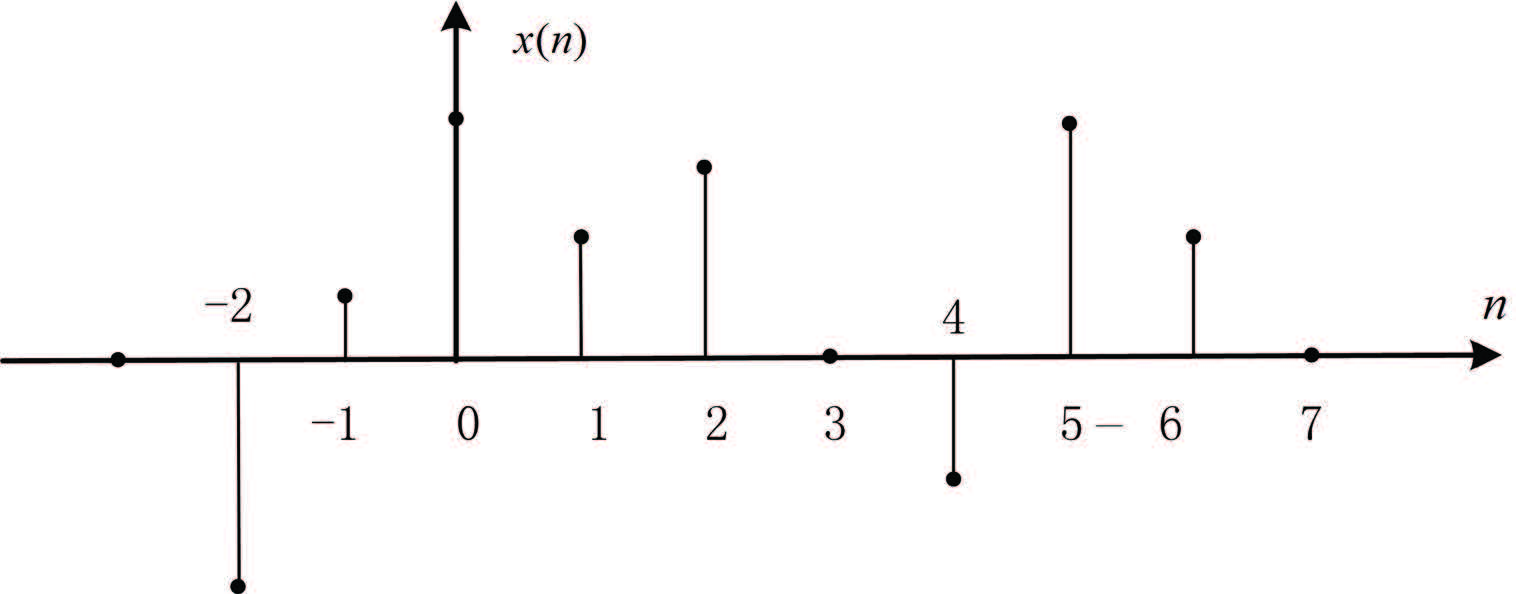
\includegraphics[width=0.6\textwidth]{yiweijiaquanhe.jpg}\\
  %\caption{用单位采样序列移位加权和表示序列}
  %\label{}
\end{figure}

显然,$x(n)$可用上述公式表示为:
$$x(n)=-2\delta(n+2)+0.5\delta(n+1)+2\delta(n)+\delta(n-1)+1.5\delta(n-2)$$
%\vspace{-0.5cm}
$$-\delta(n-4)+2\delta(n-5)+\delta(n-6)$$


\end{frame}
%%%%%%%%%%%%%%%%%%%%%%%%%%%%%%%%%%%%%%%%%%%%%%%%%%%%%%%%%%%%%%%%%%%%%%%%%%%%%%%%%%%%%%%%%%%%%%%

\section{时域离散系统}

%%%%%%%%%%%%%%%%%%%%%%%%%%%%%%%%%%%%%%%%%%%%%%%%%%%%%%%%%%%%%%%%%%%%%%%%%%%%%%%%%%%%%%%%%%%%%%
\begin{frame}\frametitle{时域离散系统}%[allowframebreaks][shrink]

设时域离散系统的输入为$x(n)$,经过规定的运算,系统输出序列用$y(n)$表示,
运算关系用$T[\cdot]$表示,输入与输出之间的关系用下式表示:
\begin{equation*}
    y(n)=T[x(n)]
\end{equation*}
\begin{figure}[h]
  \centering
  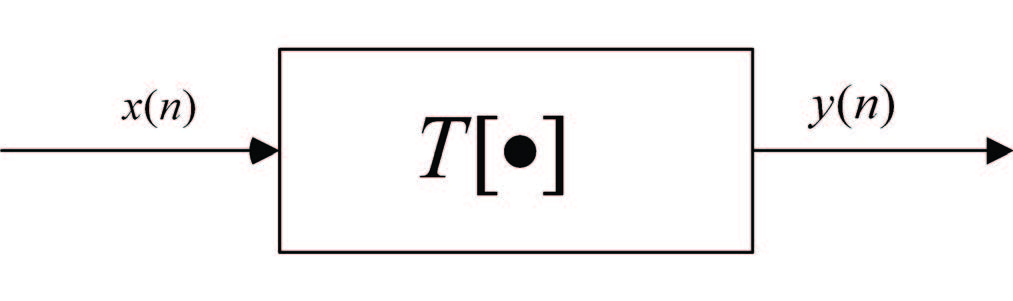
\includegraphics[width=0.6\textwidth]{shiyulisanxitong.jpg}\\
  %\caption{时域离散系统}
  %\label{}
\end{figure}
\end{frame}
%%%%%%%%%%%%%%%%%%%%%%%%%%%%%%%%%%%%%%%%%%%%%%%%%%%%%%%%%%%%%%%%%%%%%%%%%%%%%%%%%%%%%%%%%%%%%%%


\subsection{线性系统}
%%%%%%%%%%%%%%%%%%%%%%%%%%%%%%%%%%%%%%%%%%%%%%%%%%%%%%%%%%%%%%%%%%%%%%%%%%%%%%%%%%%%%%%%%%%%%%
\begin{frame}\frametitle{线性系统}%[allowframebreaks][shrink]
\begin{definition}
系统的输入输出之间满足线性叠加原理的系统称为线性系统。设$y_{1}(n)= T[x_{1}(n)]$,$y_{2}(n)= T[x_{2}(n)]$,
则线性系统必满足以下两个公式。
\begin{equation*}
     T\big[x_{1}(n)+x_{2}(n)\big] = y_{1}(n) + y_{2}(n)
\end{equation*}
\begin{equation*}
     T\big[ax_{1}(n)\big] = ay_{1}(n)
\end{equation*}
\end{definition}
也可将两个公式结合起来,写作:
\begin{equation*}
     T\big[ax_{1}(n)+bx_{2}(n)\big] = aT\big[x_{1}(n)\big]+bT\big[x_{2}(n)\big]
\end{equation*}
式中,$a$,$b$为任意常数。

简单的说,就是\textbf{和的输出等于输出的和}
\end{frame}
%%%%%%%%%%%%%%%%%%%%%%%%%%%%%%%%%%%%%%%%%%%%%%%%%%%%%%%%%%%%%%%%%%%%%%%%%%%%%%%%%%%%%%%%%%%%%%%

\subsection{时不变系统}

%%%%%%%%%%%%%%%%%%%%%%%%%%%%%%%%%%%%%%%%%%%%%%%%%%%%%%%%%%%%%%%%%%%%%%%%%%%%%%%%%%%%%%%%%%%%%%
\begin{frame}\frametitle{时不变系统}%[allowframebreaks][shrink]


\begin{definition}
\textbf{设 $y(n) = T[x(n)]$,若$y(n-n_{0})=T[x(n-n_{0})]$,则系统称为时不变系统。}
\end{definition}
\quad\newline\quad
时不变系统对输入信号的响应与输入信号加于系统的时间无关,或者说,系统的运算$T[\cdot]$不随时间变化。
%\newline\newline\newline\newline\newline\newline\newline
%\begin{center}
%时不变系统示意图
%\end{center}
%\begin{figure}[h!tbp]
%  
\includegraphics[width=0.4\textwidth]{blankpic.jpg}\\
%  %\caption{时不变系统示意图}%\label{}
%\end{figure}
\end{frame}
%%%%%%%%%%%%%%%%%%%%%%%%%%%%%%%%%%%%%%%%%%%%%%%%%%%%%%%%%%%%%%%%%%%%%%%%%%%%%%%%%%%%%%%%%%%%%%%



%%%%%%%%%%%%%%%%%%%%%%%%%%%%%%%%%%%%%%%%%%%%%%%%%%%%%%%%%%%%%%%%%%%%%%%%%%%%%%%%%%%%%%%%%%%%%%
\begin{frame}\frametitle{}%[allowframebreaks][shrink]
\begin{example}
设$y(n)=4x(n)+3$,说明其是否为线性时不变系统。%(a和b是常数)
\par\textbf{解}:
\begin{enumerate}
  \item 线性\par
        $aT[x_{1}(n)] + bT[x_{2}(n)]= 4ax_{1}(n)+3a + 4bx_{2}(n)+3b$\par
        %$y_{2}(n) = T[x_{2}(n)] = 4bx_{2}(n)+3b$\par
        $T[ax_{1}(n)+bx_{2}(n)] =  4ax_{1}(n) + 4bx_{2}(n)+3$\par
        $T[ax_{1}(n)+bx_{2}(n)] \neq  aT[x_{1}(n)] + bT[x_{2}(n)]$\par
        因此,该系统不是线性系统。
  \item 时不变性\par  %式中a和b是常数。
        $y(n) = 4x(n) +3$\par
        $y(n-n_{0}) = 4x(n-n_{0}) + 3$\par
        $T[x(n-n_{0})] =  4x(n-n_{0}) + 3$\par
        $y(n-n_{0}) = T[x(n-n_{0})]$\par
        因此该系统是时不变系统。
\end{enumerate}
\end{example}
\end{frame}
%%%%%%%%%%%%%%%%%%%%%%%%%%%%%%%%%%%%%%%%%%%%%%%%%%%%%%%%%%%%%%%%%%%%%%%%%%%%%%%%%%%%%%%%%%%%%%%



%%%%%%%%%%%%%%%%%%%%%%%%%%%%%%%%%%%%%%%%%%%%%%%%%%%%%%%%%%%%%%%%%%%%%%%%%%%%%%%%%%%%%%%%%%%%%%
\begin{frame}\frametitle{}%[allowframebreaks][shrink]
\begin{example}
检查$y(n)=nx(n)$所代表的系统是否为线性时不变系统。
\par\textbf{解}:
\begin{enumerate}
  \item 线性  \par
        $aT[x_{1}(n)] + bT[x_{2}(n)]= a n x_{1}(n) + b n x_{2}(n)$\par
        $T[ax_{1}(n)+bx_{2}(n)] = n(a x_{1}(n) + bx_{2}(n))$\par
        $T[ax_{1}(n)+bx_{2}(n)] =  aT[x_{1}(n)] + bT[x_{2}(n)]$\par
        因此,该系统是线性系统。
  \item 时不变性 \par
        $y(n) = nx(n)$\par
        $y(n-n_{0}) = (n-n_{0})x(n-n_{0})$\quad\quad  (代入n)\par
        $T[x(n-n_{0})] = nx(n-n_{0})$\quad\quad\quad\quad (代入$x(n)$ )\par
        $y(n-n_{0}) \neq T[x(n-n_{0})]$\par
        因此该系统不是时不变系统。
\end{enumerate}
\end{example}
\end{frame}
%%%%%%%%%%%%%%%%%%%%%%%%%%%%%%%%%%%%%%%%%%%%%%%%%%%%%%%%%%%%%%%%%%%%%%%%%%%%%%%%%%%%%%%%%%%%%%%

\subsection{线性时不变系统输入与输出之间的关系}
\begin{frame}[shrink]\frametitle{时域离散系统的输入输出响应}%[allowframebreaks][shrink]
%线性时不变系统: 同时满足线性和时不变特性的系统成为时域离散线性时不变系统
\begin{enumerate}
  \item 时域离散系统的输入输出响应
      \begin{itemize}
        \item \textbf{零输入响应:}仅由$n_0$时刻的初始状态或历史输入信号引起的响应称为零输入响应。
        \item \textbf{零状态响应:}仅由当前输入信号引起的响应称为零状态响应。
        \item \textbf{混合响应 :} 零输入响应和零状态响应之和称为系统的完全响应。
      \end{itemize}
  \item    单位脉冲响应$h(n)$
      %\begin{dablock}
      \begin{itemize}
        \item 系统对于单位脉冲信号$\delta(n)$的零状态响应称为单位脉冲响应,可用公式表示为:
        $$h(n) = T\big[\delta(n)\big]$$
        \item $h(n)$与模拟系统中的单位冲激响应相对应,代表系统的时域特性。
      \end{itemize}
      %\end{dablock}
\end{enumerate}


\end{frame}

\subsubsection*{线性时不变系统输入与输出之间的关系}


%%%%%%%%%%%%%%%%%%%%%%%%%%%%%%%%%%%%%%%%%%%%%%%%%%%%%%%%%%%%%%%%%%%%%%%%%%%%%%%%%%%%%%%%%%%%%%
\begin{frame}[shrink]\frametitle{线性时不变系统输入与输出之间的关系}%[allowframebreaks][shrink]
\begin{wenti}
已知线性时不变系统的单位取样响应$h(n)$,以及系统的输入信号$x(n)$,求系统的输出$y(n)$
\end{wenti}
\begin{dablock}
\begin{enumerate}
  \item []  一、单位取样响应
\end{enumerate}
\end{dablock}
$h(n)$是系统对$\delta(n)$的零状态响应,代表了系统的时域特性。
            $$h(n)=T[\delta(n)]$$
\begin{figure}[h]
  \centering
  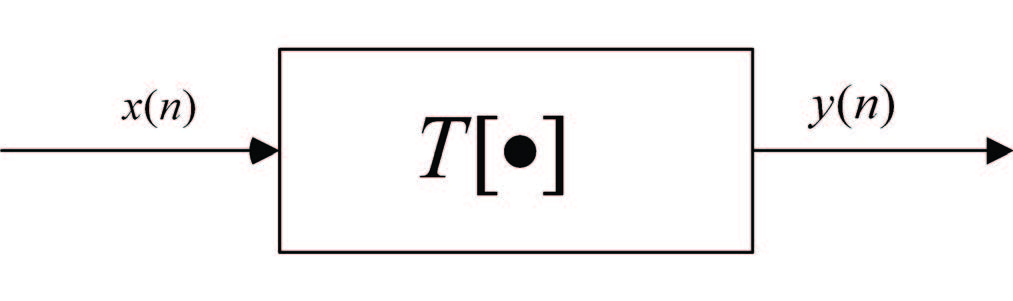
\includegraphics[width=0.5\textwidth]{shiyulisanxitong.jpg}\\
  %\caption{时域离散系统}
  %\label{}
\end{figure}


\end{frame}



%%%%%%%%%%%%%%%%%%%%%%%%%%%%%%%%%%%%%%%%%%%%%%%%%%%%%%%%%%%%%%%%%%%%%%%%%%%%%%%%%%%%%%%%%%%%%%
\begin{frame}\frametitle{}%[allowframebreaks][shrink]
\begin{dablock}
\begin{enumerate}
  \item  [] 二、卷积关系
\end{enumerate}
\end{dablock}

\begin{enumerate}
  \item [(1)] 系统输入$x(n)$可表示成单位采样序列的移位加权和:
              \begin{equation*}
                x(n) = \sum_{m=-\infty}^{\infty}x(m)\delta(n-m)
              \end{equation*}
  \item [(2)] 那么系统输出为:
                  \begin{equation*}
                  \begin{split}
                    y(n) &= T\big[x(n)\big]= T\left[\sum_{m=-\infty}^{\infty}x(m)\delta(n-m)\right]\\
                         &= \sum_{m=-\infty}^{\infty}x(m)T[\delta(n-m)] \mbox{\qquad (线性)}\\
                         &= \sum_{m=-\infty}^{\infty}x(m)h(n-m)  \mbox{\qquad (时不变性)}\\
                         &= x(n)*h(n)
                  \end{split}
                  \end{equation*}
\end{enumerate}


\end{frame}
%%%%%%%%%%%%%%%%%%%%%%%%%%%%%%%%%%%%%%%%%%%%%%%%%%%%%%%%%%%%%%%%%%%%%%%%%%%%%%%%%%%%%%%%%%%%%%%
\begin{frame}\frametitle{线性时不变系统输入与输出之间的关系}%[allowframebreaks][shrink]
\begin{dablock}
\begin{enumerate}
  \item []  \textbf{三、结论}
\end{enumerate}
\end{dablock}
\par\qquad 线性时不变系统的输出$y(n)$等于输入序列$x(n)$和系统的单位取样响应$h(n)$的卷积,该卷积
    称作线性卷积。


\end{frame}
\subsubsection*{卷积的计算}

%%%%%%%%%%%%%%%%%%%%%%%%%%%%%%%%%%%%%%%%%%%%%%%%%%%%%%%%%%%%%%%%%%%%%%%%%%%%%%%%%%%%%%%%%%%%%%
\begin{frame}[shrink]\frametitle{卷积的计算}%[allowframebreaks][shrink]

%
%\begin{enumerate}
%  \item [1] 计算公式\par
%\end{enumerate}
      \begin{enumerate}
          \item
              回忆一下模拟信号卷积公式:
              $$y(t) = x(t)*h(t) = \int_{-\infty}^{\infty}x(\tau)h(t-\tau)d\tau $$\par
              离散信号卷积公式:
              $$y(n) = x(n)*h(n) = \sum_{m=-\infty}^{\infty}x(m)h(n-m)$$\par
          \item 计算方法 \par
              \qquad 与模拟系统中的连续卷积计算很类似,即反褶(翻转)、移位、相乘、相加。
%              \begin{enumerate}
%                \item 翻转: $h(m)\rightarrow h(-m)$
%                \item 移位:固定一个n的值,$h(-m)\rightarrow h(n-m)$
%                \item 相乘:$x(m)\cdot h(n-m)$
%                \item 相加:$\sum_{m=-\infty}^{\infty}x(m)h(n-m)$
%              \end{enumerate}
      \end{enumerate}
\end{frame}
%%%%%%%%%%%%%%%%%%%%%%%%%%%%%%%%%%%%%%%%%%%%%%%%%%%%%%%%%%%%%%%%%%%%%%%%%%%%%%%%%%%%%%%%%%%%%%%



%%%%%%%%%%%%%%%%%%%%%%%%%%%%%%%%%%%%%%%%%%%%%%%%%%%%%%%%%%%%%%%%%%%%%%%%%%%%%%%%%%%%%%%%%%%%%%
\begin{frame}\frametitle{}%[allowframebreaks][shrink]
\begin{example}
    设$x(n)=R_{4}(n)$,$h(n)=R_{3}(n)$,求$y(n)=x(n)*h(n)$。
\end{example}

\begin{dablock}
计算过程:反褶(翻转)、移位、相乘、相加。
              \begin{enumerate}
                \item 翻转: $h(m)\rightarrow h(-m)$
                \item 移位:固定一个n的值,$h(-m)\rightarrow h(n-m)$
                \item 相乘:$x(m)\cdot h(n-m)$
                \item 相加:$\sum_{m=-\infty}^{\infty}x(m)h(n-m)$
              \end{enumerate}
\end{dablock}
\end{frame}
%%%%%%%%%%%%%%%%%%%%%%%%%%%%%%%%%%%%%%%%%%%%%%%%%%%%%%%%%%%%%%%%%%%%%%%%%%%%%%%%%%%%%%%%%%%%%%%


\subsubsection*{卷积的性质}

%%%%%%%%%%%%%%%%%%%%%%%%%%%%%%%%%%%%%%%%%%%%%%%%%%%%%%%%%%%%%%%%%%%%%%%%%%%%%%%%%%%%%%%%%%%%%%
\begin{frame}\frametitle{卷积的性质}%[allowframebreaks][shrink]
%\begin{description}
%  \item[] 
%\end{description}

\begin{enumerate}
  \item[(1)] 卷积服从交换律、结合律、分配律,即:
  \begin{dablock}
            \begin{equation*}
                x(n)*y(n) = y(n)*x(n)
            \end{equation*}

            \begin{equation*}
                x(n)*\big(y(n)*\omega(n)\big) = \big(x(n)*y(n)\big)*\omega(n)
            \end{equation*}

            \begin{equation*}
                x(n)*\big(y(n)+\omega(n)\big) = x(n)*y(n)+x(n)*\omega(n)
            \end{equation*}
 \end{dablock}
\end{enumerate}
\end{frame}

\begin{frame}\frametitle{卷积的性质}%[allowframebreaks][shrink]
\begin{enumerate}
  \item[(2)]  关于系统级联与并联的等效系统
         \begin{dablock}
            \begin{enumerate}
               \item 两个系统级联,其单位取样响应相当于两个系统各自单位取样响应卷积。
               \item 两个系统并联,其单位取样响应相当于两个系统各自单位取样响应求和。
               \item 但该结论仅限于线性时不变系统,对于非线性或时变系统,这些结论不成立。
            \end{enumerate}
          \end{dablock}
\end{enumerate}
\end{frame}



\begin{frame}\frametitle{卷积的性质}%[allowframebreaks][shrink]
\begin{enumerate}
  \item [(3)]  序列与$\delta(n-n_{0})$的线性卷积
         \begin{dablock}
         序列与移位的单位取样响应$\delta(n-n_{0})$的线性卷积相当于将序列本身移位$n_{0}$,
      如下式所示:$$x(n-n_{0})=x(n)*\delta(n-n_{0})$$
      \end{dablock}
\end{enumerate}

\end{frame}
%%%%%%%%%%%%%%%%%%%%%%%%%%%%%%%%%%%%%%%%%%%%%%%%%%%%%%%%%%%%%%%%%%%%%%%%%%%%%%%%%%%%%%%%%%%%%%%





%%%%%%%%%%%%%%%%%%%%%%%%%%%%%%%%%%%%%%%%%%%%%%%%%%%%%%%%%%%%%%%%%%%%%%%%%%%%%%%%%%%%%%%%%%%%%%
\begin{frame}[shrink]\frametitle{}%[allowframebreaks][shrink]
\begin{example}
在下图中,$h_{1}(n)$系统与$h_{2}(n)$系统级联,设,
$x(n)=u(n)$,
$h_{1}(n)=\delta(n)-\delta(n-4)$,
$h_{2}(n)=a^{n}u(n)\quad(|a|<1)$,
求系统的输出$y(n)$.
\end{example}
%
\begin{figure}[h]
\centering
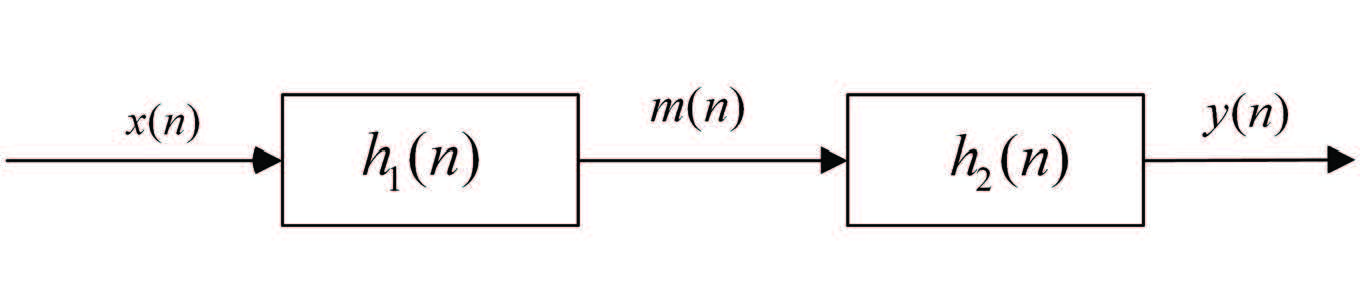
\includegraphics[width=0.6\textwidth]{li135.jpg}\\
%\caption{例1.3.5框图}
%\label{}
\end{figure}

解:先求第一级的输出$m(n)$,再求$y(n)$。
\begin{dablock}
\begin{equation*}
\begin{split}
    m(n)  &= x(n)*h_{1}(n)= u(n)*[\delta(n)-\delta(n-4)]\\
          &=u(n)*\delta(n) - u(n)*\delta(n-4)=u(n)-u(n-4) \\
          &= R_{4}(n)\\
\end{split}
\end{equation*}
\end{dablock}
然后有:
\begin{dablock}
\begin{equation*}
\begin{split}
    y(n) &= m(n)*h_{2}(n) = R_{4}(n)*a^{n}u(n)\\
%         &=a^{n}u(n)*[\delta(n)+\delta(n-1)+\delta(n-2)+\delta(n-3)]\\
%         &=a^{n}u(n)+a^{n-1}u(n-1)+a^{n-2}u(n-2)+a^{n-3}u(n-3)\\
\end{split}
\end{equation*}
\end{dablock}

%还可以将$y(n)$用下式表示:\par
%$y(n)=\delta(n)+(1+a)\delta(n-1)+(a+a+a^{2})\delta(n-2) + [a^{n}\sum_{k=0}^{3}a^{-k}]u(n-3)$

\end{frame}
%%%%%%%%%%%%%%%%%%%%%%%%%%%%%%%%%%%%%%%%%%%%%%%%%%%%%%%%%%%%%%%%%%%%%%%%%%%%%%%%%%%%%%%%%%%%%%%



\subsection{系统的因果性与稳定性}

%\begin{frame}[allowframebreaks]\frametitle{系统的因果性和稳定性}%[allowframebreaks][shrink]

%\end{frame}

\subsubsection*{系统的因果性}
%%%%%%%%%%%%%%%%%%%%%%%%%%%%%%%%%%%%%%%%%%%%%%%%%%%%%%%%%%%%%%%%%%%%%%%%%%%%%%%%%%%%%%%%%%%%%%
\begin{frame}[shrink]\frametitle{系统的因果性}%[allowframebreaks][shrink]

\begin{definition}
    如果系统在第n时刻的输出,仅取决于n时刻及以前的输入序列,而和n时刻以后的输入序列无关,则称该系统具有因果性质,或称该系统为因果系统。因果性实际上是指系统的可实现性。
\end{definition}
\end{frame}

\begin{frame}[shrink]\frametitle{系统的因果性}%[allowframebreaks][shrink]
\begin{theorem}{线性时不变系统具有因果性的充要条件为:}
%系统的因果性的充要条件
\begin{center}
系统因果 $\Longleftrightarrow$ $\quad h(n) =0,\quad n<0 $
\end{center}
\end{theorem}

%\begin{shuoming}
%\begin{enumerate}
%     \item 因果序列:满足上式的序列称为因果序列,因此因果系统的单位取样响应$h(n)$必是因果序列。
%     \item 因果系统的单位取样响应是必是因果序列
%\end{enumerate}
%\end{shuoming}

\end{frame}

%\begin{frame}[shrink]\frametitle{线性时不变系统具有因果性充要条件的证明}%[allowframebreaks][shrink]
%\begin{theorem}{线性时不变系统具有因果性的充要条件为:}
%%系统的因果性的充要条件
%\begin{center}
%系统因果 $\Longleftrightarrow$ $\quad h(n) =0,\quad n<0 $
%\end{center}
%\end{theorem}
%
%\end{frame}



\begin{frame}[shrink]\frametitle{}
\begin{daproof}
充分性:($\Leftarrow$) 假设$h(n)=0$,$n<0$,往证系统因果。

% ($\Leftarrow$) 假设$h(n)=0$,$n<0$,往证系统因果。\par
%        \quadquad\quad 因为 %\vspace{-0.5cm}
        $$%\qquad\mbox{因为}  \qquad
        y(n) = x(n) * h(n)%=\sum_{m=-\infty}^{\infty}x(m)h(n-m)
                =\sum_{m=-\infty}^{\infty}h(m)x(n-m) $$%\vspace{-0.5cm}
            \quad\quad 令$n=n_{0}$,则
        $$y(n_{0})=\sum_{m=-\infty}^{\infty}h(m)x(n_{0}-m)$$%= \sum_{m=-\infty}^{\infty}x(m)h(n_{0}-m)
        \quad\quad 又,\quad$h(n)=0$,$n<0$,则有
        $$y(n_{0}) = \sum_{m=0}^{\infty}h(m)x(n_{0}-m)$$
        \quad\quad 显然: $n_{0}-m \leqslant n_{0}$
        \quad\quad 由定义知,系统是因果的。\par
\end{daproof}
\end{frame}

\begin{frame}[shrink]\frametitle{}
 \begin{daproof}
必要性($\Rightarrow$) 假设系统因果,往证 $h(n)=0$,$n<0$。

  %($\Rightarrow$) 假设系统因果,往证 $h(n)=0$,$n<0$。
  $$\because\qquad  %\mbox{因为}  \qquad
        y(n) = x(n) * h(n)%=\sum_{m=-\infty}^{\infty}x(m)h(n-m)
                =\sum_{m=-\infty}^{\infty}h(m)x(n-m) $$%\vspace{-0.5cm}
        $$\therefore \qquad y(n_{0}) = \sum_{m=-\infty}^{\infty}h(m)x(n_{0}-m)\quad\quad\quad$$
        $$\therefore \quad y(n_{0}) = \sum_{m=-\infty}^{-1}h(m)x(n_{0}-m) + \sum_{m=0}^{\infty}h(m)x(n_{0}-m)$$

        \par \textbf{分析:}
        \par 若系统为因果,当$m<0$时,$x(n_0-m)$在$y(n_0)$之后发生,与系统因果性定义矛盾,
        此时必有$h(n)=0$,$n<0$,才不令此情况发生。
        $$\therefore \quad\quad\quad h(n)=0,n<0\quad\quad\quad$$

\end{daproof}

\end{frame}
%%%%%%%%%%%%%%%%%%%%%%%%%%%%%%%%%%%%%%%%%%%%%%%%%%%%%%%%%%%%%%%%%%%%%%%%%%%%%%%%%%%%%%%%%%%%%%
\begin{frame}[shrink]\frametitle{线性时不变系统具有因果性充要条件的证明}%[allowframebreaks][shrink]


\begin{shuoming}
\begin{enumerate}
     \item 因果序列 \par
           \begin{center}
           $x(n)$是因果序列  $\Longleftrightarrow$ $\quad x(n) =0,\quad n<0 $
           \end{center}
     \item 因果系统的单位取样响应是必是因果序列
\end{enumerate}
\end{shuoming}



\end{frame}

\subsubsection*{系统的稳定性}
%%%%%%%%%%%%%%%%%%%%%%%%%%%%%%%%%%%%%%%%%%%%%%%%%%%%%%%%%%%%%%%%%%%%%%%%%%%%%%%%%%%%%%%%%%%%%%
\begin{frame}[shrink]\frametitle{系统稳定的定义}%[allowframebreaks][shrink]
\begin{definition}

        所谓稳定系统,指系统输入有界,则系统输出也有界,即:
        \begin{equation*}
          \mbox{若}|x(n)|< \infty\quad\Longrightarrow\quad |y(n)|<\infty
        \end{equation*}
\end{definition}
\end{frame}


\begin{frame}[shrink]\frametitle{线性时不变系统稳定的充要条件}%[allowframebreaks][shrink]
\begin{theorem}
   线性时不变系统稳定的充要条件%\vspace{-0.5cm}
        \begin{center}
        系统稳定  $\Longleftrightarrow$ 系统的单位取样响应绝对可和,即
        \end{center}%\vspace{-0.5cm}
        \begin{equation*}        \sum_{n=-\infty}^{\infty}|h(n)|<\infty
        \end{equation*}%\vspace{-0.5cm}
   \end{theorem}



\end{frame}

\begin{frame}[shrink]\frametitle{}%[allowframebreaks][shrink]

1. 充分性($\Longleftarrow$)
\begin{daproof}
设输入序列为$x(n)$,输出序列为$y(n)$,则有:
            $$y(n) = \sum_{k=-\infty}^{\infty}h(k)x(n-k)$$
            $$|y(n)| \leq \sum_{k=-\infty}^{\infty}|h(k)||x(n-k)|$$
            因为输入序列$x(n)$有界,即必存在某一常数$B$,使得
            $|x(n)|<B,\quad -\infty<n<\infty$,
            因此:
            $$|y(n)| \leq B\sum_{k=-\infty}^{\infty}|h(k)| <\infty$$
            如果系统的单位取样响应$h(n)$满足上式,
            那么输出$y(n)$一定也是有界的,即:$y(n)<\infty$.
\end{daproof}
\end{frame}

\begin{frame}[shrink]\frametitle{}%[allowframebreaks][shrink]
2. 必要性$(\Longrightarrow)$
\begin{daproof}
   如果$h(n)$不满足原条件。既$\sum_{k=-\infty}^{\infty}|h(n)|=\infty$,那么总可以找到一个有界的输入引起无界的输出。

   例如,我们可以构造一个输入序列使得输出无界。
            \begin{equation*}
                 x(n)= \left\{\begin{array}
                 {r@{,\quad}l}
                 \frac{h^{*}(-n)}{|h(-n)|}&\mbox{$h(n)\neq0$}\\0&\mbox{$h(n)=0$}
                \end{array} \right.
            \end{equation*}

            $$\mbox{则有:}\qquad y(n) = \sum_{k=-\infty}^{\infty}h(k)x(n-k)$$

            令$n=0$,
            $$y(0) = \sum_{k=-\infty}^{\infty}h(k)x(0-k) = \sum_{k=-\infty}^{\infty}h(k)\frac{h^{*}(k)}{|h(k)|} = \sum_{k=-\infty}^{\infty}|h(k)| = \infty$$
            上式说明$n=0$时刻的输出为无穷大,系统不稳定,从而证明了其必要性。
\end{daproof}
\end{frame}
%%%%%%%%%%%%%%%%%%%%%%%%%%%%%%%%%%%%%%%%%%%%%%%%%%%%%%%%%%%%%%%%%%%%%%%%%%%%%%%%%%%%%%%%%%%%%%%



%%%%%%%%%%%%%%%%%%%%%%%%%%%%%%%%%%%%%%%%%%%%%%%%%%%%%%%%%%%%%%%%%%%%%%%%%%%%%%%%%%%%%%%%%%%%%%
\begin{frame}\frametitle{}%[allowframebreaks][shrink]
\begin{example}

设线性时不变系统的单位取样响应$h(n)=a^{n}u(n)$,式中a是实常数,试分析
该系统的因果稳定性。
\end{example}
\par\textbf{解}:\par
\begin{enumerate}
  \item 因果性
        \par 由于$n<0$时,$h(n)=0$,所以系统是因果系统。\par
  \item 稳定性
           $$\sum_{n=-\infty}^{\infty}|h(n)|= \sum_{n=0}^{\infty}|a|^{n} = \lim_{N\rightarrow\infty}\sum_{n=0}^{N-1}|a|^{n} = \lim_{N\rightarrow\infty}\frac{1-|a|^{N}}{1-|a|}$$
        只有当$|a|<1$时,
           $$\sum_{n=-\infty}^{\infty}|h(n)| = \frac{1}{1-|a|}$$
        因此系统稳定的条件是$|a|<1$
\end{enumerate}

\end{frame}
%%%%%%%%%%%%%%%%%%%%%%%%%%%%%%%%%%%%%%%%%%%%%%%%%%%%%%%%%%%%%%%%%%%%%%%%%%%%%%%%%%%%%%%%%%%%%%%



%%%%%%%%%%%%%%%%%%%%%%%%%%%%%%%%%%%%%%%%%%%%%%%%%%%%%%%%%%%%%%%%%%%%%%%%%%%%%%%%%%%%%%%%%%%%%%%
%\begin{frame}[allowframebreaks]\frametitle{}%[allowframebreaks][shrink]
%\begin{example}
%设系统的单位取样响应$h(n)=u(n)$,求对任意输入序列$x(n)$的输出$y(n)$,并
%检验系统的因果性和稳定性。
%\end{example}
%\par\textbf{解}:依题意,显然有 $h(n)=u(n)$
%$$y(n) = x(n)*\mu(n) = \sum_{k=-\infty}^{\infty}x(k)u(n-k)$$
%
%因为当\quad $n-k<0$时,$u(n-k)=0$; 而$n-k\geq0$时,$u(n-k)=1$, 因此,求和限为$k\leq n$,所以
%$$y(n)=\sum_{k=-\infty}^{n}x(k)$$
%
%上式表明该系统是一个累加器,它将输入序列从加上之时开始,逐项累加到n 时为止。
%\par下 面分析该系统的稳定性,由于
%$$\sum_{n=-\infty}^{\infty}|h(n)| = \sum_{n=0}^{\infty}|u(n)| = \infty$$
%
%因此该系统是一个不稳定系统。显然该系统为一个因果系统。
%
%\end{frame}
%%%%%%%%%%%%%%%%%%%%%%%%%%%%%%%%%%%%%%%%%%%%%%%%%%%%%%%%%%%%%%%%%%%%%%%%%%%%%%%%%%%%%%%%%%%%%%%%


\section{采样定理}
%%%%%%%%%%%%%%%%%%%%%%%%%%%%%%%%%%%%%%%%%%%%%%%%%%%%%%%%%%%%%%%%%%%%%%%%%%%%%%%%%%%%%%%%%%%%%%
\begin{frame}[shrink]\frametitle{模拟信号的数字处理方法}%[allowframebreaks][shrink]
\qquad 为利用计算机对模拟信号进行处理,人们需要将模拟信号经过采样和量化形成数字信号,通过数字信号处理方法处理完毕后,在转换为模拟信号。
这种方法称为模拟信号的数字处理方法。\par
\qquad  在此过程中,一个关键问题就是对模拟信号的采样过程。
\newline
\begin{wenti}
\begin{enumerate}
  \item 理想采样信号频谱与原模拟信号频谱的关系是什么?
  \item 为了使得采样信号能不失真的恢复原模拟信号,采样角频率$\Omega_s$与信号最高频率$\Omega_c$的关系是什么?
\end{enumerate}
\end{wenti}

\end{frame}
%%%%%%%%%%%%%%%%%%%%%%%%%%%%%%%%%%%%%%%%%%%%%%%%%%%%%%%%%%%%%%%%%%%%%%%%%%%%%%%%%%%%%%%%%%%%%%%
%%%%%%%%%%%%%%%%%%%%%%%%%%%%%%%%%%%%%%%%%%%%%%%%%%%%%%%%%%%%%%%%%%%%%%%%%%%%%%%%%%%%%%%%%%%%%%
\begin{frame}\frametitle{采样信号$\hat{x}_a(t)$的得到}%[allowframebreaks][shrink]
设$x_a(t)$为模拟信号,$\hat{x}_a(t)$为采样信号, $p_{\delta}(t)$为单位冲击串。
%$$\mbox{且有}\quad\quad   p_{\delta}(t)= \sum_{n=-\infty}^{\infty}\delta(t-nT)$$

%\begin{align*}%\label{}
%  x_a(t)          &:\mbox{模拟信号}  \\
%  p_{\delta}(t)   &:\mbox{单位冲击串}\quad\quad p_{\delta}(t)=
%                     \sum_{n=-\infty}^{\infty}\delta(t-nT)  \\
%  \hat{x}_a(t)    &: \mbox{采样信号}
%\end{align*}
\begin{dablock}
采样信号$\hat{x}_a(t)$可看做模拟信号$x_a(t)$和单位冲击串$p_{\delta}(t)$相乘
$$\hat{x}_a(t) =  x_a(t)\cdot p_{\delta}(t)$$
%
\end{dablock}
$$   p_{\delta}(t)= \sum_{n=-\infty}^{\infty}\delta(t-nT),\mbox{且仅在$t=nT$处有非0值。}$$
\begin{equation*}
\begin{split}
\hat{x}_a(t)   &= x_a(t)\cdot p_{\delta}(t) =  \sum_{n=-\infty}^{\infty} x_a(t)\cdot \delta(t-nT) \\
               &=  \sum_{n=-\infty}^{\infty} x_a(nT)\cdot \delta(t-nT)
\end{split}
\end{equation*}
\end{frame}


\begin{frame}[shrink]\frametitle{推导}%[allowframebreaks][shrink]
\begin{dablock}
\begin{align*}%\label{}
  \mbox{设:}\quad x_a(t)
          &\leftrightarrow  X_a(j\Omega)\quad\quad\quad\quad\quad\quad\quad\quad\quad\quad\quad\quad  \\
  p_{\delta}(t)
          &\leftrightarrow  P_{\delta}(j\Omega)   \\
  \mbox{则:}\quad x_a(t)\cdot p_{\delta}(t)
          &\leftrightarrow  \frac{1}{2\pi}X_a(j\Omega)*P_{\delta}(j\Omega)
\end{align*}
\end{dablock}

\begin{equation*}
\begin{split}
  P_{\delta}(j\Omega)
         &=  FT\left[\sum_{n=-\infty}^{\infty}\delta(t-nT)\right]
                      \quad\quad\quad\quad\quad\quad\quad\quad\\
         &=  \frac{2\pi}{T}\sum_{k=-\infty}^{\infty}\delta(\Omega- k \Omega_s)
             \quad\quad\quad \mbox{注意这里 \quad }\Omega_s = \frac{2\pi}{T}
\end{split}
\end{equation*}
\end{frame}



\begin{frame}[shrink]\frametitle{推导}%[allowframebreaks][shrink]
\begin{equation*}
\begin{split}
  \hat{X}_a(j\Omega)
         &=  FT\left[\hat{x}_a(t)\right] = FT\left[x_a(t)\cdot p_{\delta}(t) \right]
                      \quad\quad\quad\quad\quad\quad\quad\quad\\
         &=  \frac{1}{2\pi}X_a(j\Omega) * P_{\delta}(j\Omega)\\
         &=  \frac{1}{2\pi}\cdot \frac{2\pi}{T}\int_{-\infty}^{\infty}X_a(j\theta)\cdot
             \sum_{k=-\infty}^{\infty}\delta(\Omega- k \Omega_s-\theta)d\theta \\
         &=  \frac{1}{T}\sum_{k=-\infty}^{\infty}\int_{-\infty}^{\infty}
             X_a(j\theta)\cdot \delta(\Omega - k \Omega_s-\theta) d\theta \\
         &=  \frac{1}{T}\sum_{k=-\infty}^{\infty}X_a(j\Omega -j k \Omega_s)
             \quad\quad\quad \left(\int_{-\infty}^{\infty}f(t)\delta(t-t_0)dt = f(t_0)\right)\qquad
\end{split}
\end{equation*}
$$\therefore \quad\quad
\hat{X}_a(j\Omega)   =  \frac{1}{T}\sum_{k=-\infty}^{\infty}X_a(j\Omega -k \Omega_s)
\quad\quad\quad\quad\quad\quad\quad\quad\quad\quad
$$
\end{frame}
%
%
%
\begin{frame}[shrink]\frametitle{说明}%[allowframebreaks][shrink]
\textbf{说明:}
\begin{enumerate}
  \item
      理想采样信号的频谱是原信号的频谱沿频率轴每间隔采样角频率$\Omega_s$重复出现一次,并叠加形成的周期函数。
      \newline%\newline\newline\newline\newline\newline
      \begin{dablock}
        假设信号$f(t)$是一个带限信号,$\Omega_c$是信号的最高频率,则:
          \begin{itemize}
            \item 当$\Omega_s \geq 2\Omega_c$时,频谱没有混叠现象,可恢复原信号。
            \item 当$\Omega_s < 2\Omega_c$时,频谱存在混叠现象,不可能恢复原信号。
          \end{itemize}
      \end{dablock}
  \item
      实际的信号不可能为有限带宽,总存在一定的频率混叠现象。%如下图所示:
      \newline%\newline\newline\newline\newline\newline
      此时可对信号做预处理,将高于$\frac{\Omega_s}{2}$的高频信号滤去。
\end{enumerate}

\end{frame}
%%%%%%%%%%%%%%%%%%%%%%%%%%%%%%%%%%%%%%%%%%%%%%%%%%%%%%%%%%%%%%%%%%%%%%%%%%%%%%%%%%%%%%%%%%%%%%%%
%


%%%%%%%%%%%%%%%%%%%%%%%%%%%%%%%%%%%%%%%%%%%%%%%%%%%%%%%%%%%%%%%%%%%%%%%%%%%%%%%%%%%%%%%%%%%%%%
%\begin{frame}\frametitle{title}%[allowframebreaks][shrink]
%
%\end{frame}
%%%%%%%%%%%%%%%%%%%%%%%%%%%%%%%%%%%%%%%%%%%%%%%%%%%%%%%%%%%%%%%%%%%%%%%%%%%%%%%%%%%%%%%%%%%%%%%


\end{document}

